\documentclass[a4paper,12pt]{article}

\usepackage{graphicx}
\usepackage{epsfig,subfigure}
\usepackage[%dvipdfm,
            CJKbookmarks=true,%
            bookmarksnumbered=true,
            bookmarksopen=true, %Collapse all bookmarks at pdf start view
            pdfauthor=kmc,
            pdfcreator={LaTex with hyperref package},
            pdftitle=trudge,
            colorlinks,%
            linkcolor=blue,%
            hyperindex,%
            plainpages=false,%
            pdfstartview=FitH,
            linktocpage=true,
            citecolor=blue,
            hyperindex=true
            ]{hyperref}
\usepackage{listings}
\lstset{language=C}

\addtolength{\textwidth}{50pt}
\addtolength{\evensidemargin}{-25pt}
\addtolength{\oddsidemargin}{-25pt}

\def\displayandname#1{\rlap{$\displaystyle\csname #1\endcsname$}%
                      \qquad \texttt{\char92 #1}}
\def\mathlexicon#1{$$\vcenter{\halign{\displayandname{##}\hfil&&\qquad
                   \displayandname{##}\hfil\cr #1}}$$}

\newpage
\begin{document}

\title{CertiKOS Development  Notes}
%\author{Liang Gu}
%\date{2nd Edition\\[3pt]
%Copyright \copyright\ David R. Wilkins 1995}
\maketitle

\tableofcontents

\newpage
\section{About CertiKOS }

CertiKOS (Certified Kit Operating System) may refer to our project: applying new advances
in certified software \cite{certifiedsoftware} to the development of a novel OS kernel. For more information about the whole project, please check  the project tech report \cite{CertiKOSReport}. In this document, we mostly use CertiKOS to refer to the prototype of the OS kernel.

For the long term,  our CertiKOS is supposed to offer features as follows: safe and application-specific extensibility, provable security properties with information flow control, and accountability and recovery from hardware or application failures. The implementation will have different stages to provide these features. At current stage, CertiKOS is trying to provide some demonstration features (Section \ref{sec:currentstage}). This document will be updated later with the progress of implementation.


\section{CertiKOS at Current Stage}
\label{sec:currentstage}


\subsection{Overview}
\begin{figure}[!ht]
 \centerline{
 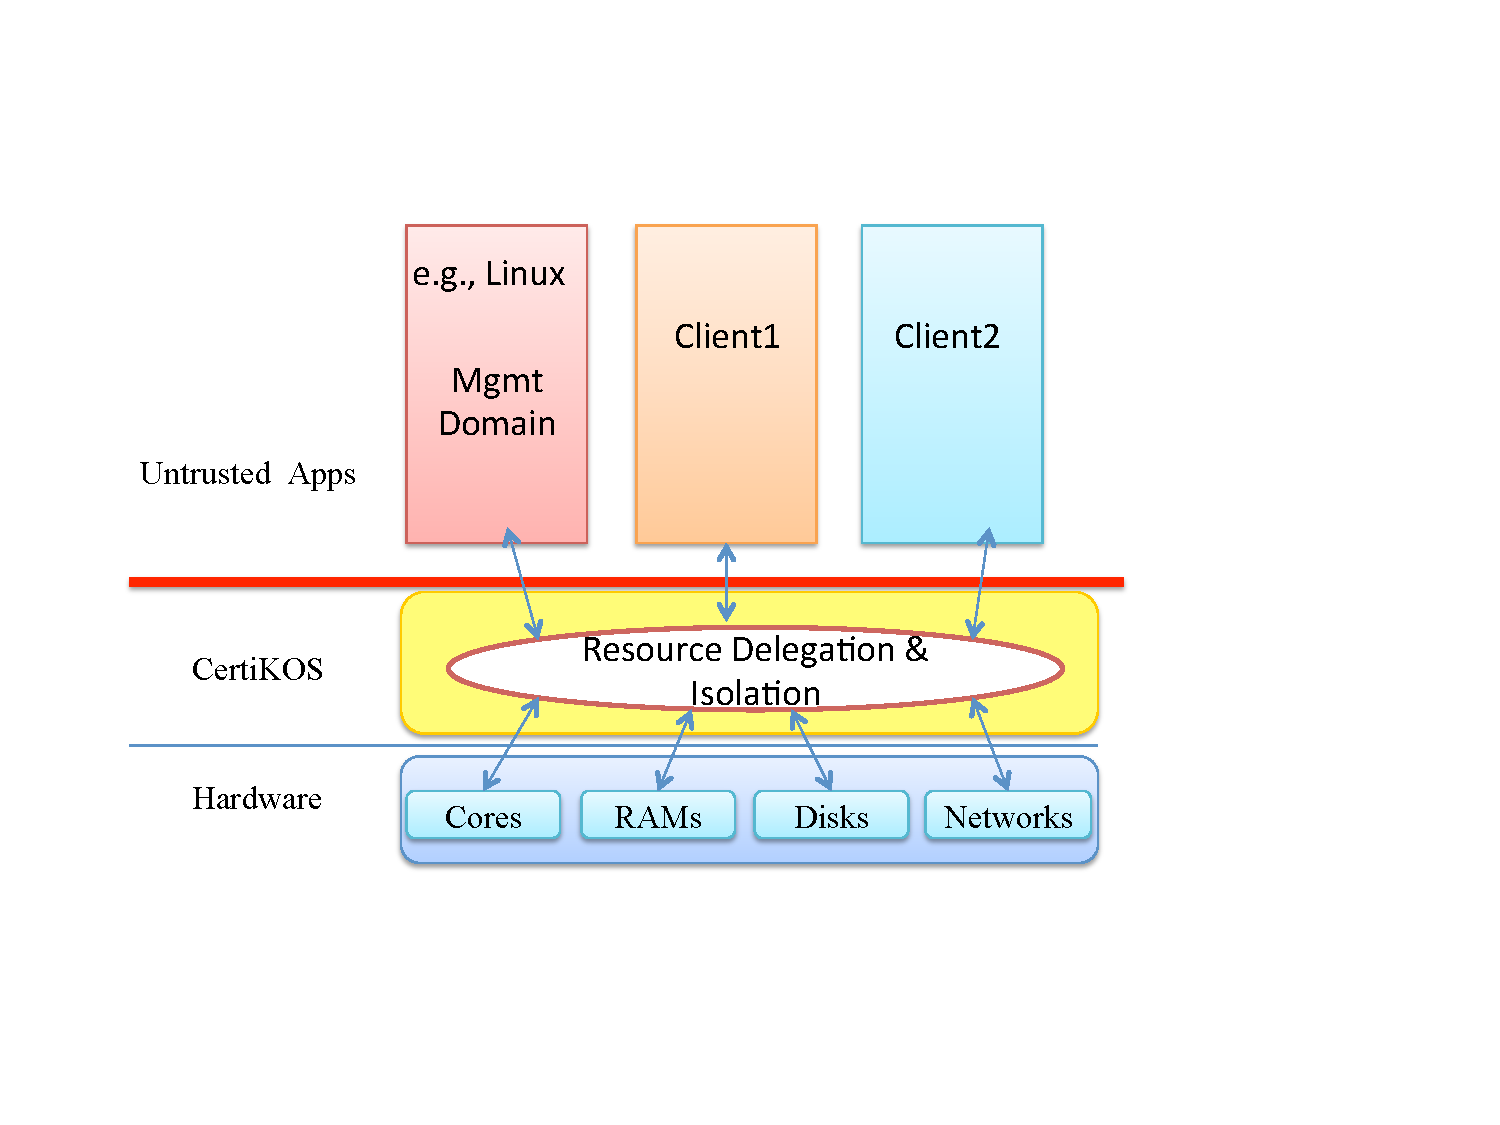
\includegraphics[width=0.6\textwidth]{overview.pdf}}
 \caption{Overview of CertiKOS at current stage} \label{fig:overview}
\end{figure}

The overview of current CertiKOS  is shown in Figure \ref{fig:overview}.  It is trying to provide demonstration features as follows:
\begin{itemize}
\item  Abstract resources for cloud computing, including CPU cores, RAMs, Disk, and Networks
\item  Separate the resource management from usage, move resource management facilities up to the untrusted application layer
\item  Support legacy OS as the management software
\item  Provide isolated execution environment to protect the execution of mission-critical (or security sensitive) operations,  according to the request from the application layer processes.
\end{itemize}

\subsection{Typical Usages }
We use several usage cases to specifically explain these above features.

\subsubsection{Resource Management}
Manage software runs at the untrusted application layer and it provides interfaces for administrator to manage the allocation of resources to each application.  As shown in Figure \ref{fig:resourcemgmt}, manage software instructs  CertiKOS to allocate  or revoke resources for applications.   Each application will be authorized to access its own resources, including memory space, cpu cores, disk and network.
\begin{figure}[!ht]
 \centerline{
 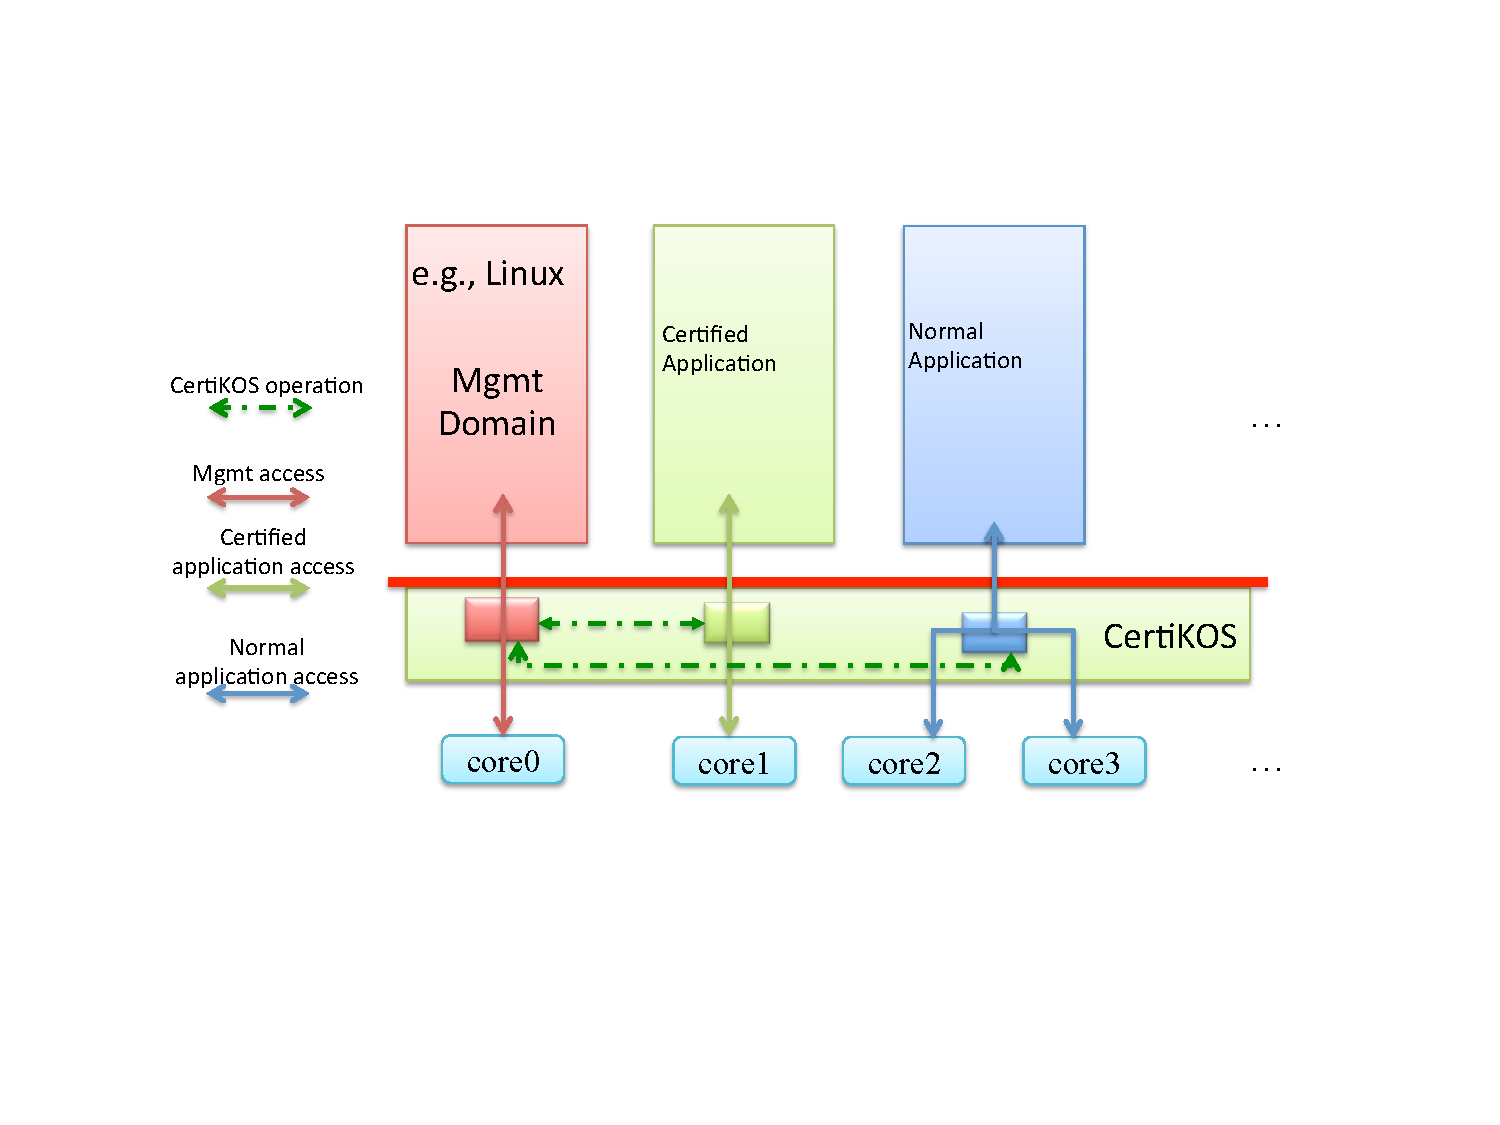
\includegraphics[width=0.7\textwidth]{certikos_resource_mgmt}}
 \caption{Resource Management} \label{fig:resourcemgmt}
\end{figure}


\subsubsection{Isolation}

Protect applications from each other, including management software.  The management software and other applications are equally treated as untrusted applications. As shown in Figure \ref{fig:isolation}, CertiKOS separately allocates memory spaces for them  and they can only access their own space.  The management software can manage the ownership of these resources, but it can not access these resources.   Applications are protected from each other and accessing among each other are prohibited.
\begin{figure}[!ht]
 \centerline{
 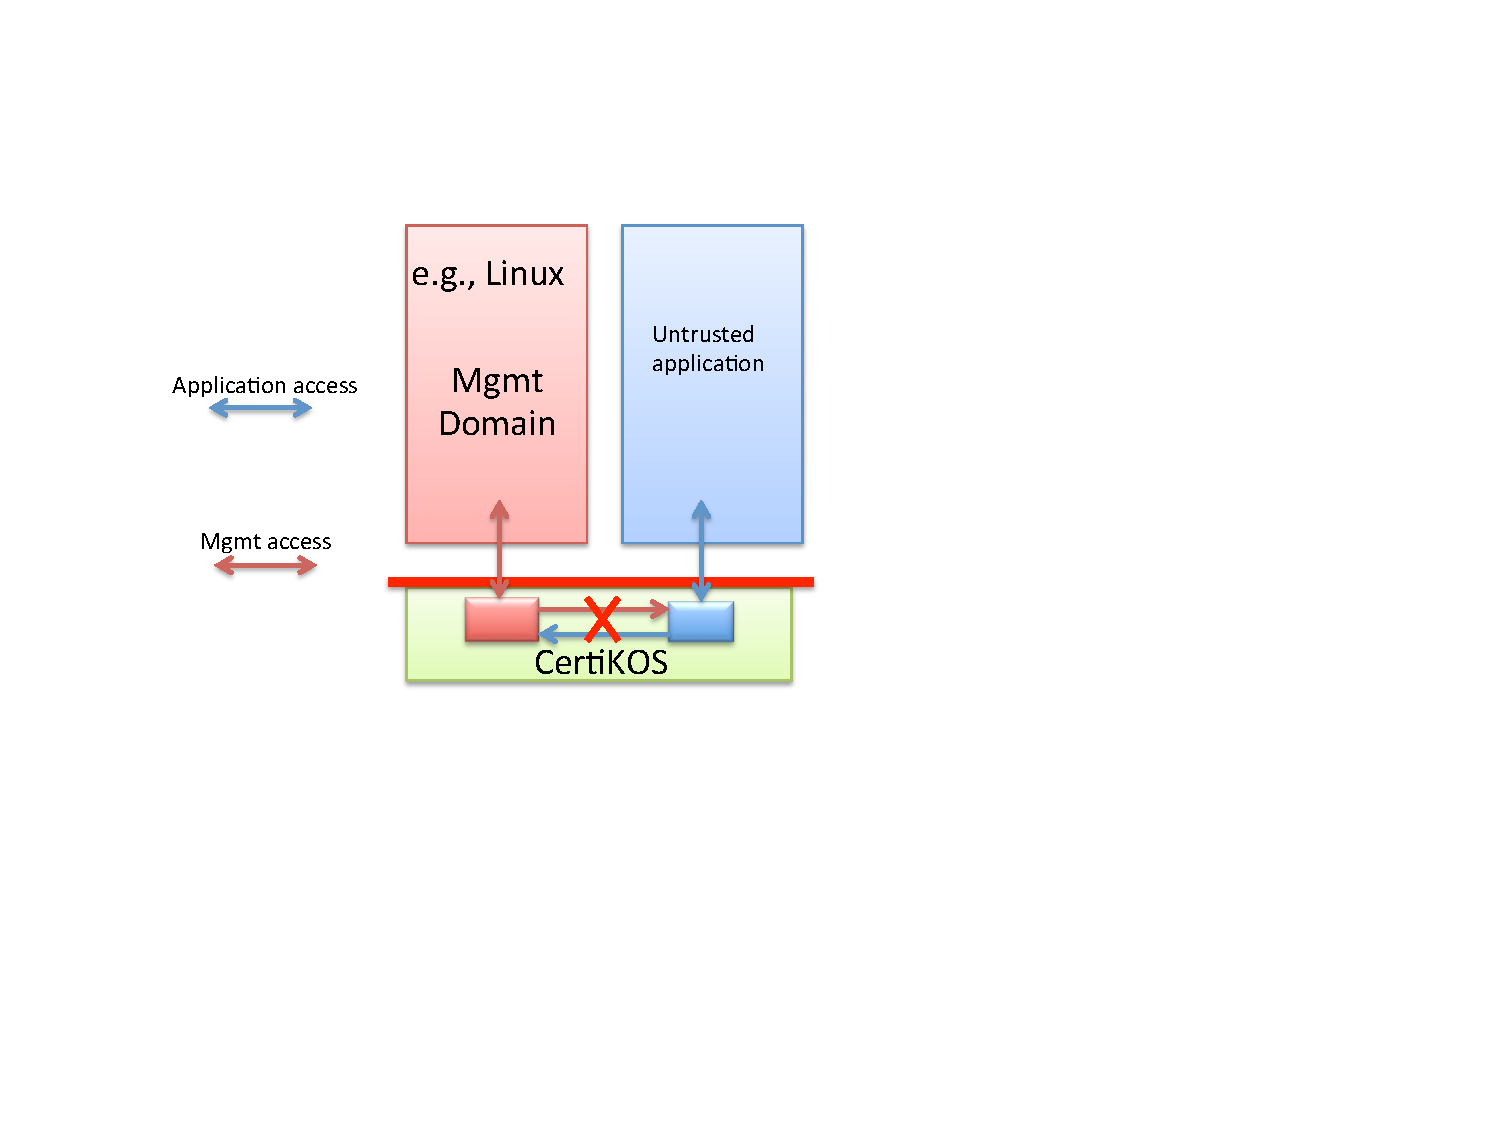
\includegraphics[width=0.4\textwidth]{certikos_isolation}}
 \caption{Isolation among untrusted applications} \label{fig:isolation}
\end{figure}

\subsubsection{Execute Certified Applications}
As shown in Figure \ref{fig:certified_ap}, certified applications can run on top of CertiKOS as normal applications and it will be protected from the management software and other applications.

\begin{figure}[!ht]
 \centerline{
 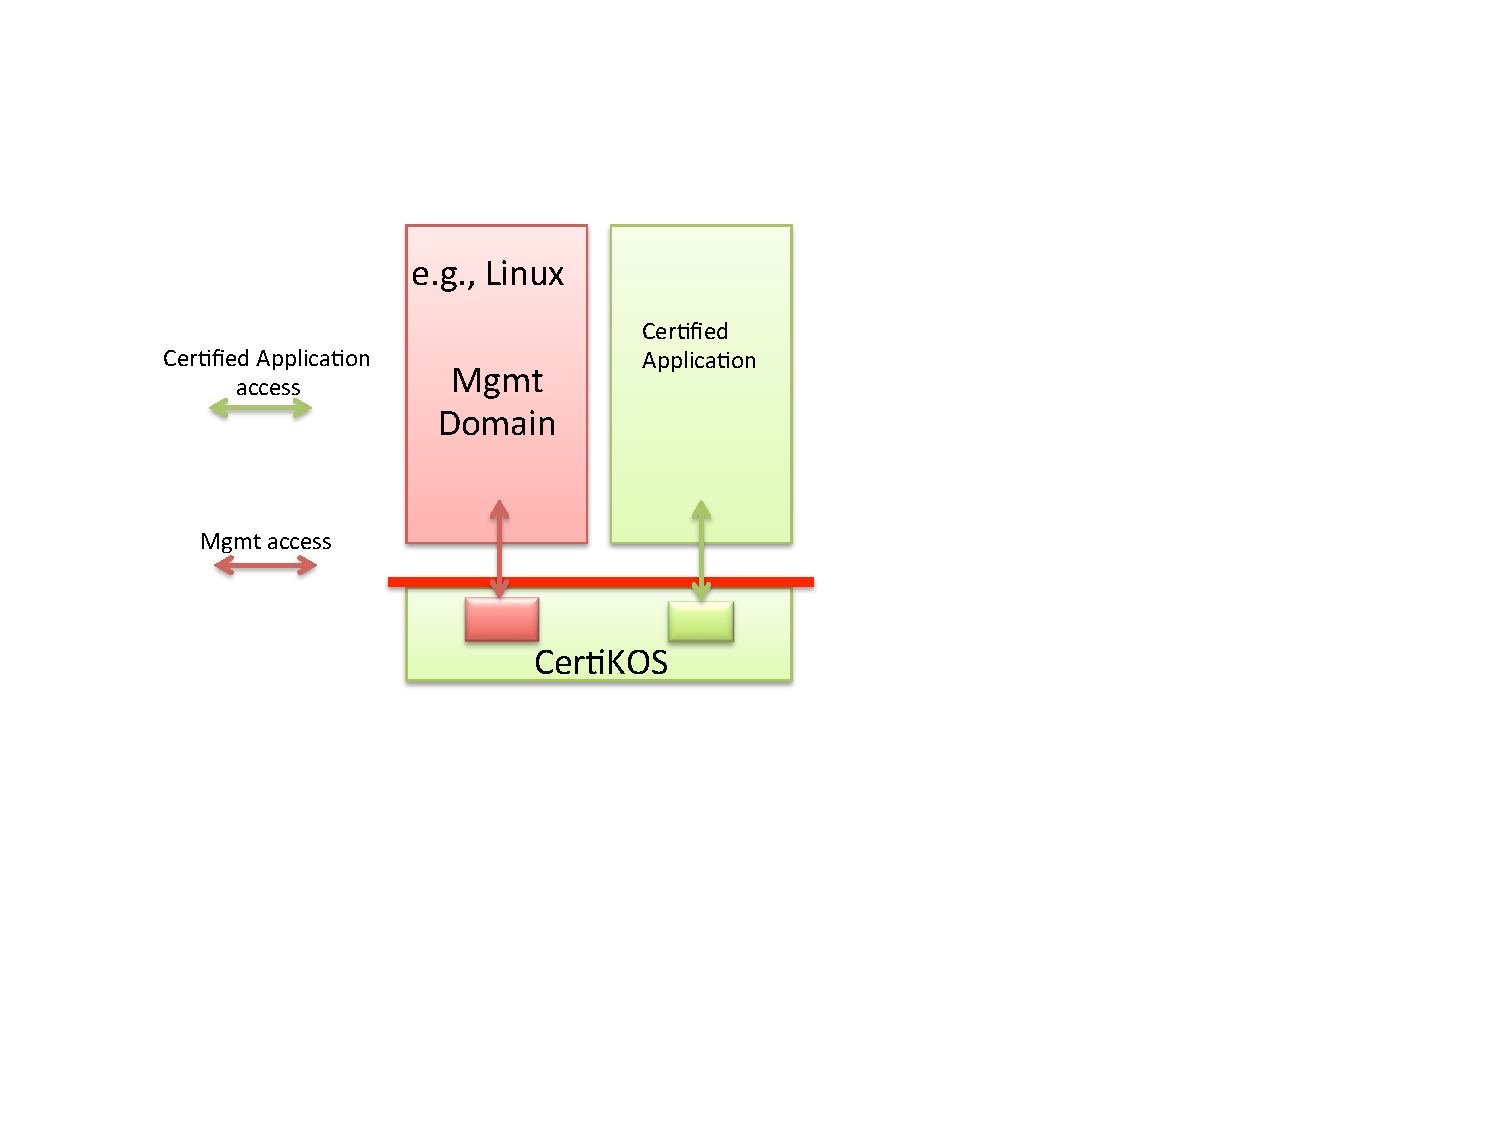
\includegraphics[width=0.4\textwidth]{certikos_certified_ap}}
 \caption{Certified Application on CertiKOS} \label{fig:certified_ap}
\end{figure}

\subsubsection{Protect Security Operations in Applications}
Many applications involve security related operations, in which sensitive information might be revealed, such as private key, credit card number,  social security number, etc. These applications may run atop of untrusted OS, and these security information can not be protected from compromised OS.

With Hardware-based Virtualization support, CertiKOS can provides isolated execution environment for these security related operations.  As shown in Figure \ref{fig:sandbox}, The legacy OS and applications can run on top of CertiKOS.  When the application tries to execute security sensitive operations,  CertiKOS  will setup a separated space for the security code block to execute.  After finishing execution in the isolated space, CertiKOS will return the result to the application and it  will continue execution in the legacy OS.



\begin{figure}[!ht]
 \centerline{
 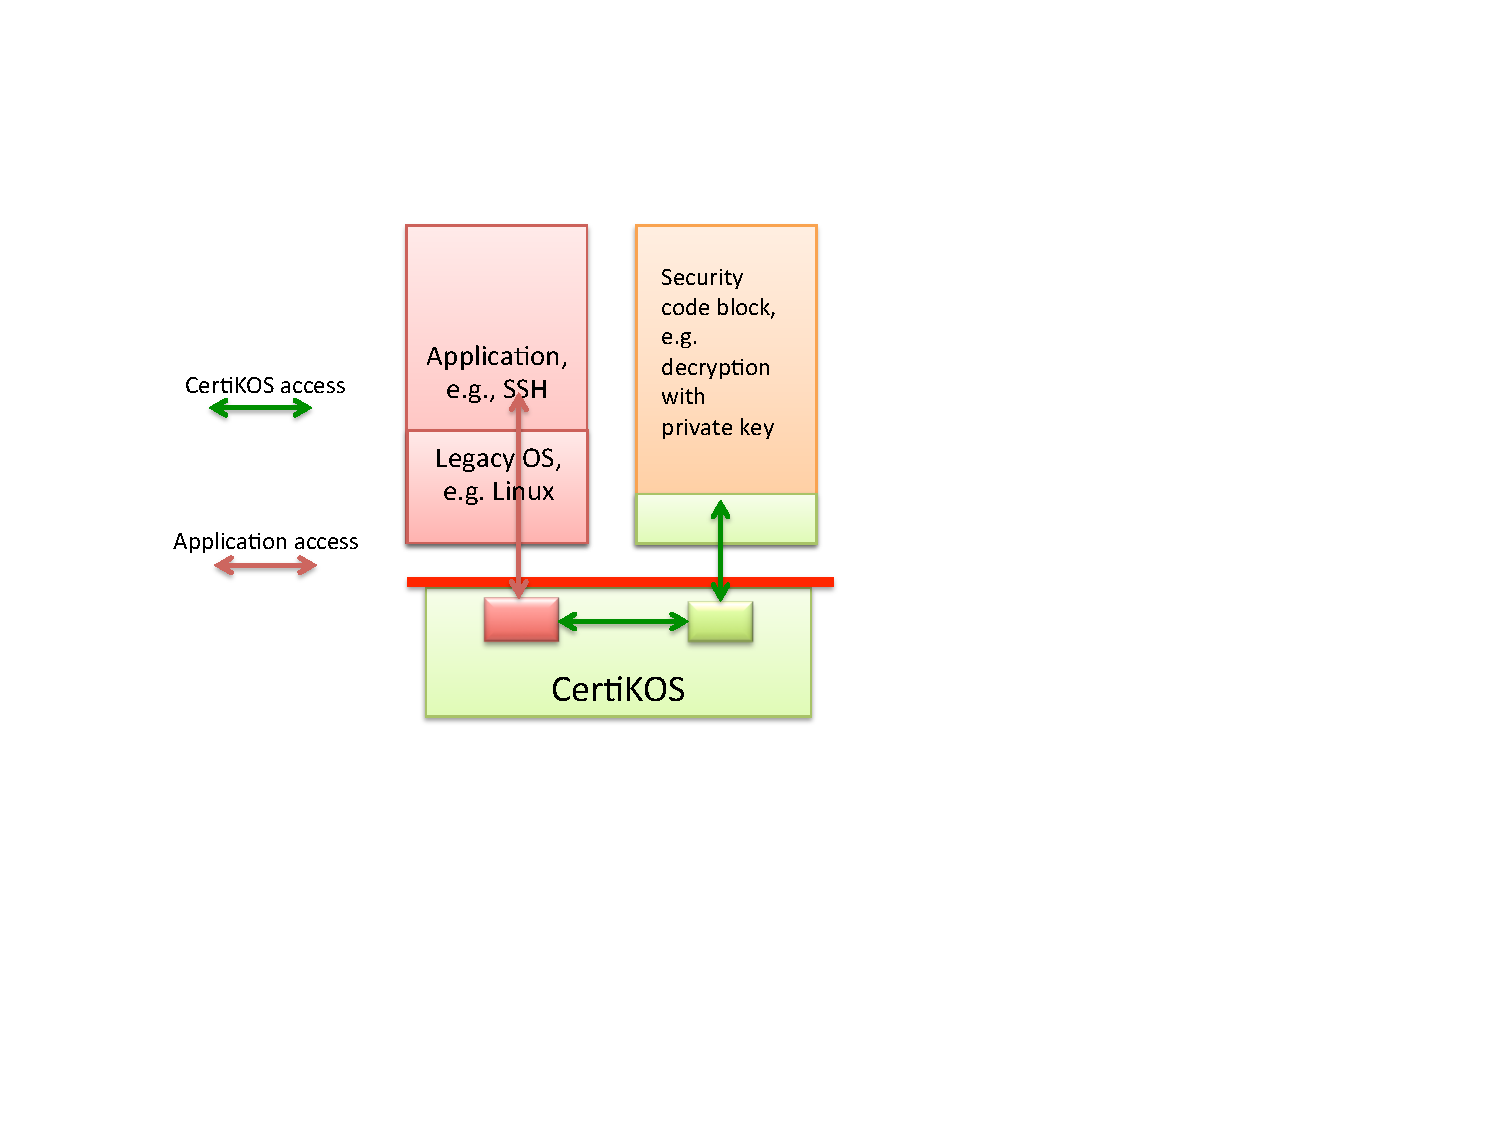
\includegraphics[width=0.4\textwidth]{certikos_sandbox}}
 \caption{Isolated Execution for Security Operations of Applications} \label{fig:sandbox}
\end{figure}

\section{CertiKOS Implementation}

\subsection{CertiKOS Framework}

\begin{figure}[!ht]
 \centerline{
 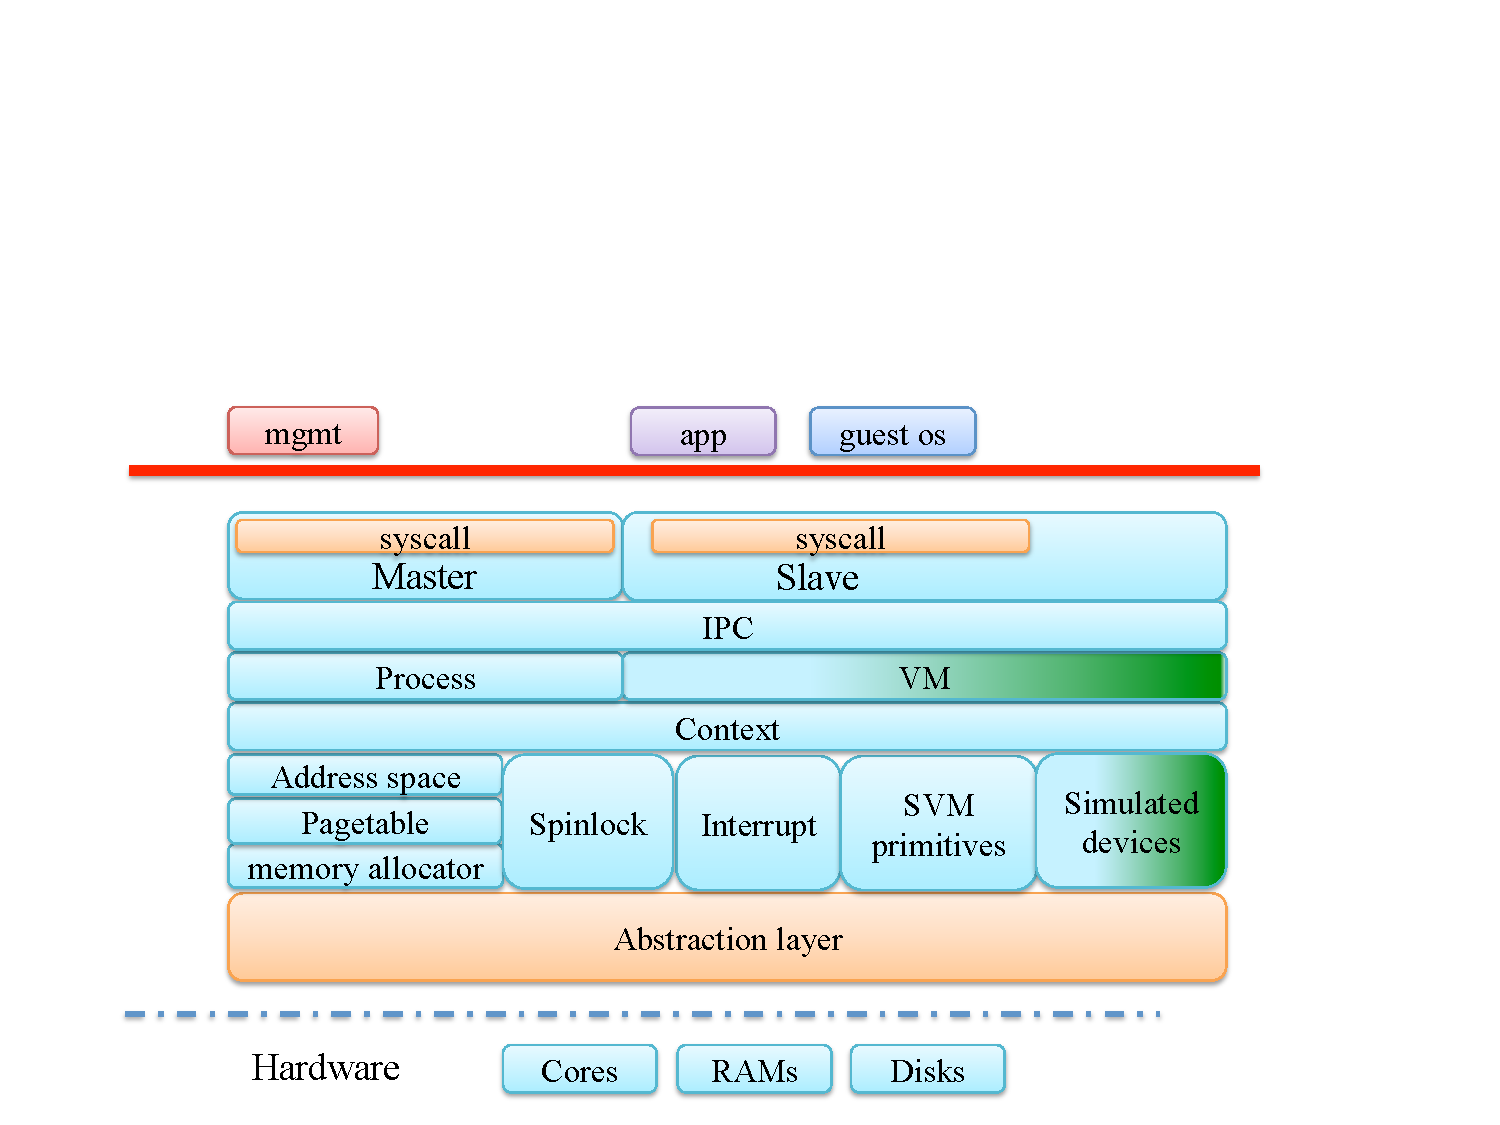
\includegraphics[width=0.8\textwidth]{certikos_framework}}
 \caption{CertiKOS Framework} \label{fig:framework}
\end{figure}

Current version of CertiKOS  is organized as in Figure \ref{fig:framework}. Upper layers depend on(invoke) lower layers components.  Ported from PIOS \cite{PIOS}, CertiKOS can now support the management of normal processes. To support legacy OS as the management software, CertiKOS takes advantage of the Hardware-based Virtualization to construct a virtualized platform space. The current implementation work is mostly focusing on SVM based virtualization support for legacy OS.  These components with mixed colors of Green and Blue denotes these undergoing implementation.

\subsection{Physical Memory Management}

Current implementation of CertiKOS uses the same way as PIOS to manage the physical memory space.  The memory space for the guest domain (VM)  consists of two parts.   The lower physical memory region from 0x0 to 0x100000 is mapped from the host memory region.  The other part of the memory space is mapped from the free memory region of CertiKOS.  For more detail, please check code files: kern/arch/i386/mem.c and kern/hvm/svm/vm.c

 \begin{figure}[!ht]
 \centerline{
 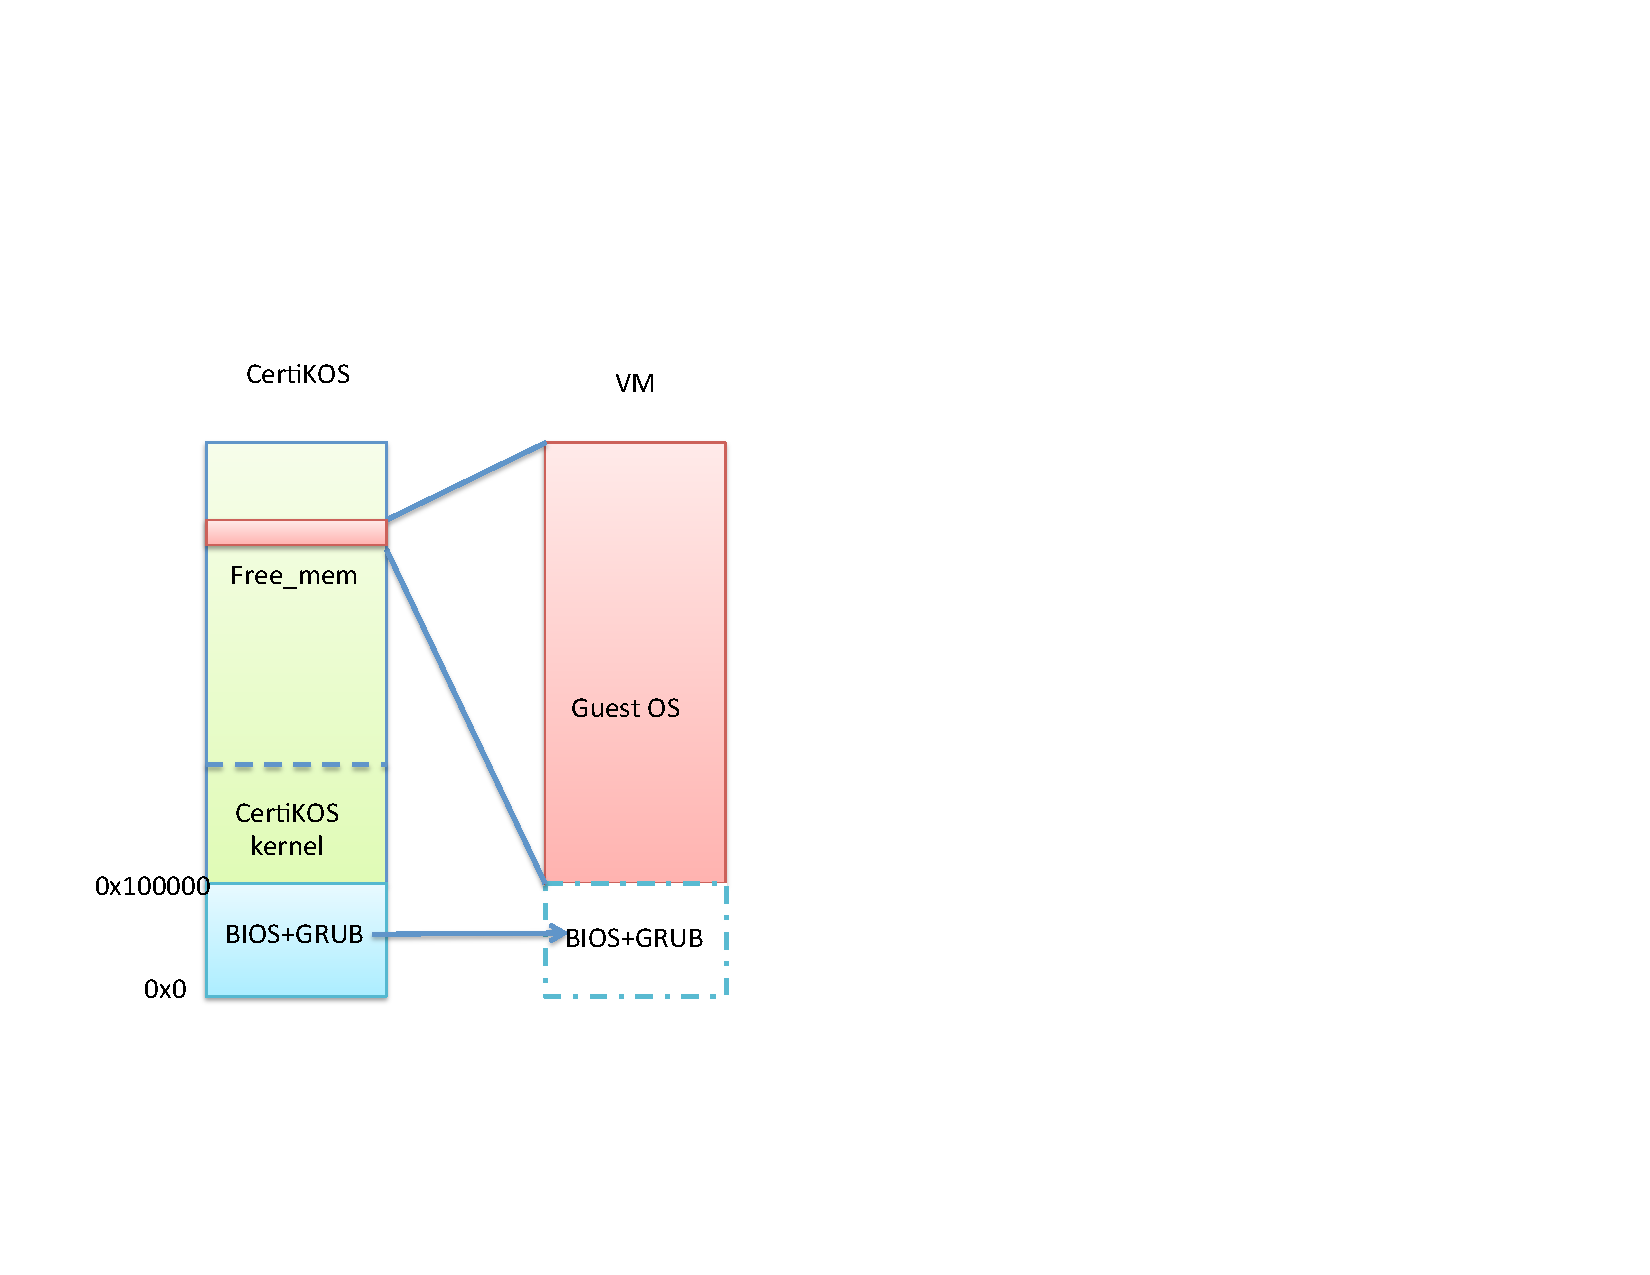
\includegraphics[width=0.6\textwidth]{physical_memory}}
 \caption{Physical Memory Layout in CertiKOS } \label{fig:phymem}
\end{figure}
\subsection{CPU Core Management}
The scheduling of processes in CertiKOS can be manually  controlled by the management shell.  CertiKOS uses a timer interrupt  handler on the bootstrap core  to examine the request list from the management shell.  If a process is assigned to run on specified core, then the timer interrupt will update the status of the target process.  Meanwhile, one all these application cores,  they repeatedly check  whether they are assigned with any process. If yes, the application core starts to execute the  given process. 

These relate codes are in files: kern/master.c and kern/slave.c.


\subsection{  Virtualization in CertiKOS}
AMD SVM provides the processor instruction support to enhance the implementation of Virtual Machine Monitor (VMM). These key features for virtualization support in CertiKOS include:  Nested Paging,  Interception,  Interrupt injection.  This subsection will briefly introduce some of these key functionalities and explain their usages in CertiKOS. For more details, please check specification \cite{AMD64, AMDSVM}.  Related codes are mostly placed under the directory of kern/hvm/svm.

\subsubsection{Virtual Machine Control}
The execution of Virtual Machine in CertiKOS is managed by the cooperations of following parts: VMCB, VMRUN, VM interception.   

VMCB  (Virtual Machine Control Block ) is the most important data structure in SVM.  It records all status information of the guest to run, including processor registers, interrupts, etc.   VMCB is basically a 4-Kbyte-aligned page that describes a virtual machine to be executed.  Addressed as a physical memory region, VMCB is usually loaded as a parameter with RAX(EAX in 32-bit mode) for the VMRUN instruction.  With VMRUN, the processor loads all status information recorded in VMCB into registers and continue to execute the instruction specified in RIP of VMCB. The VMM controls the  execution, resumption and interception of the guest os by setting the VMCB accordingly.  For more details, please refer to the Chapter 15 in  \cite{AMD64}.

\begin{figure}[!ht]
 \centerline{
 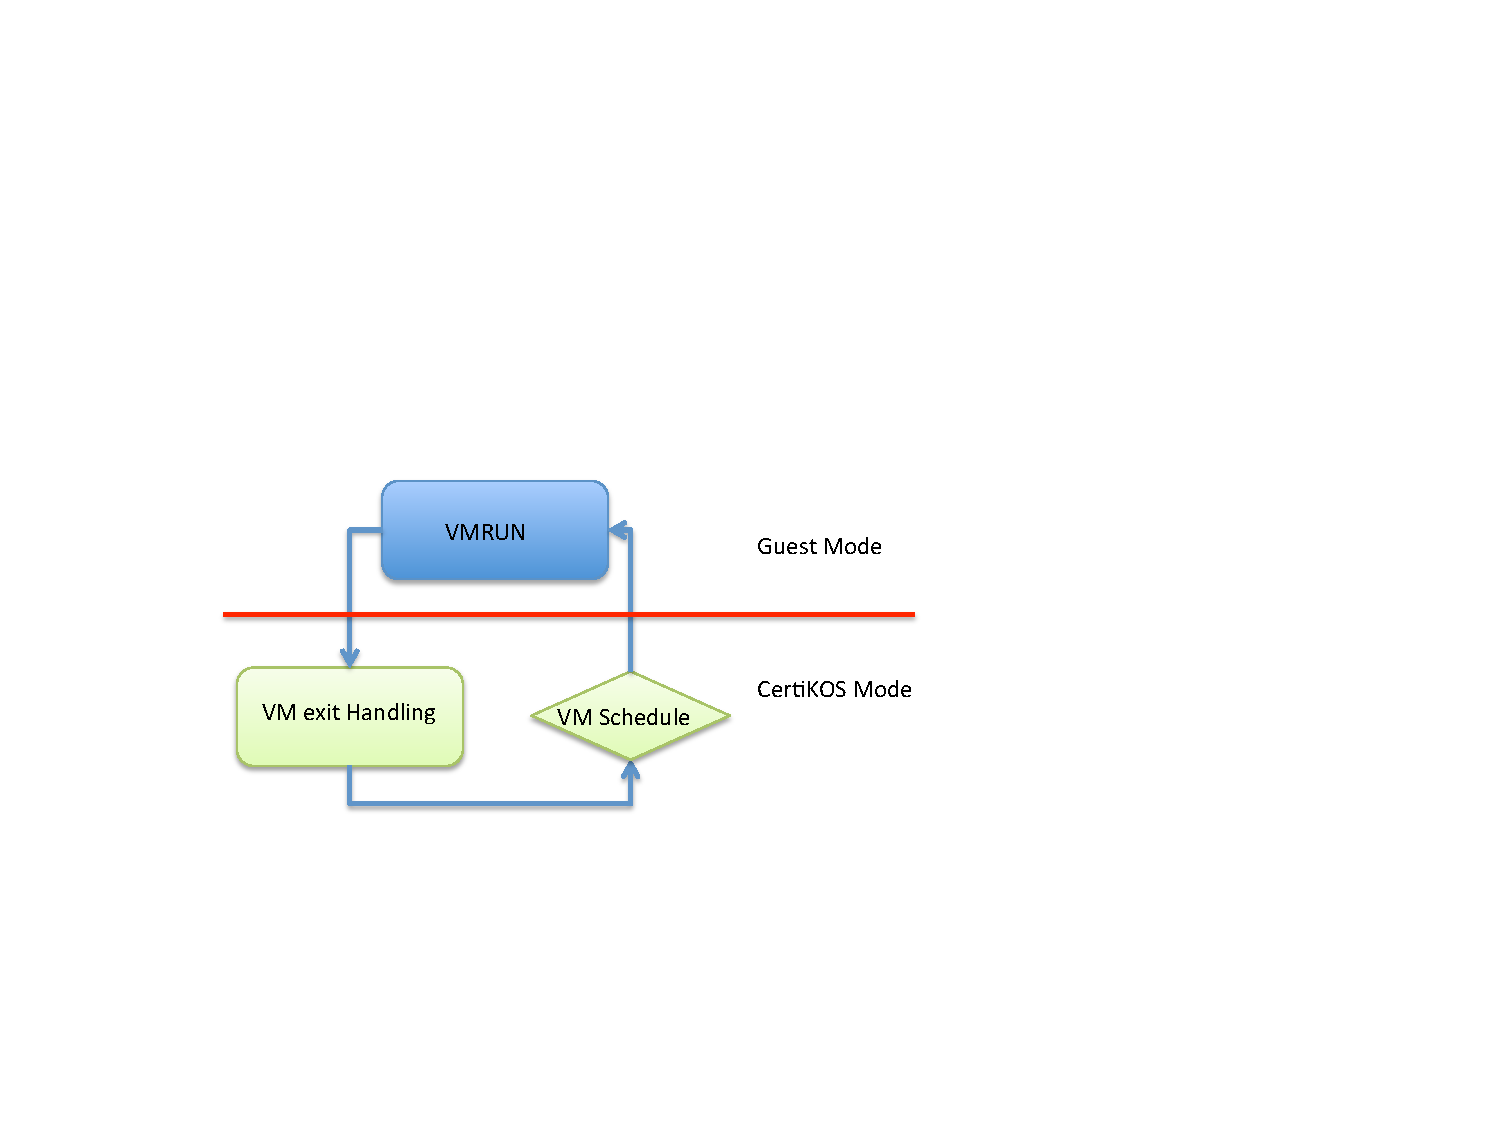
\includegraphics[width=0.6\textwidth]{vm_flow}}
 \caption{Execution Flow of VMs} \label{fig:vmflow}
\end{figure}


The basic execution flow of AMD SVM based VMM is shown as in Figure \ref{fig:vmflow}.When a VM is scheduled to run, its VMCB address will  be transferred to VMRUN instruction. Then the VMRUN will continue the execution of the VM, until exceptions or interception happen in the VM.   VM exit Handling will specifically deal with the exit event according to its exit code. After the exit handling, the VM will be ready for scheduling again.  The main control function of virtualization control is in file:kern/hvm/svm/vm.c:start\_vm().

\subsubsection{Platform Configuration for the Guest}



Previously, we directly expose all hardware to the guest domain.  This way could not support multiple VM guests. If the guest changes the BIOS setting, CertiKOS will not be able to run correctly.   So we need to identify these critical devices which might result conflicts between the Guest and CertiKOS. 

In current  CertiKOS, guest OS can only see the virtualized PIC and other interrupt chips are not provided. So we need to customize the platform  configuration  presented to the guest OS.  CertiKOS can intercept the CPUID instruction in guest domain and return a processor model with only PIC to guest domain.  So guest domain will be boot up with only PIC. To support guest OS with multi physical cores, we need to later implement the simulation of APIC and IOAPIC.

As shown in Figure \ref{fig:phymem}, the guest domain reuses the memory region of BIOS and GRUB.  In the guest domain, CertiKOS currently supposes that it starts execution from the entry address of bootloader: 0x7C00. The GRUB is responsible for loading the guest OS into its space. 

    

\subsubsection{Nested Paging}
With Nested Paging in SVM, VMM does not  have to maintain a shadow page table for the guest OS.  VMM can construct a nested page table, which maps the guest physical memory address to the host physical address.

\begin{figure}[!ht]
 \centerline{
 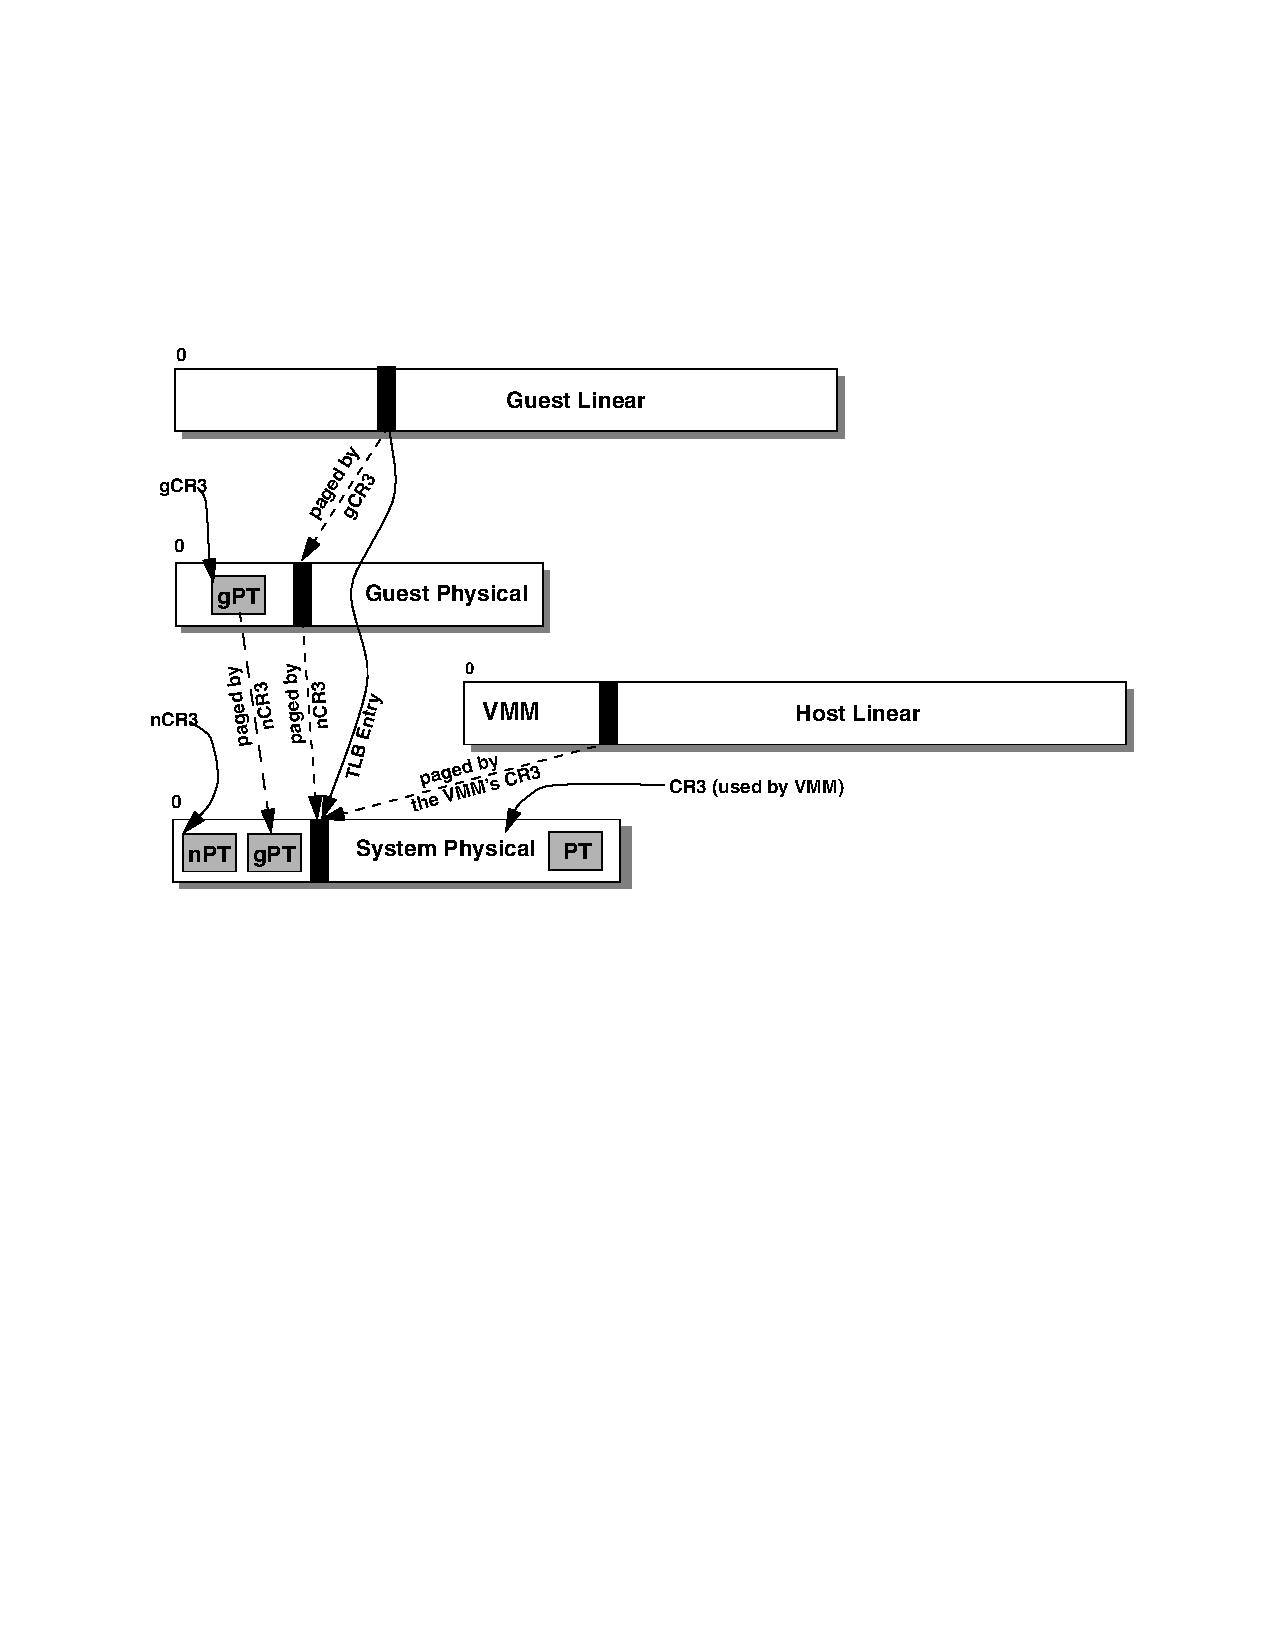
\includegraphics[width=0.8\textwidth]{NestedPaging}}
 \caption{Address Translating with Nested Paging} \label{fig:nestedpaging}
\end{figure}

With nested paging enabled, two levels of address translation are applied; Shown as in Figure \ref{fig:nestedpaging}.

\begin{itemize} \item Both guest and host levels have their own copy of CR3, referred to as gCR3 and nCR3,
respectively.
\item Guest page tables (gPT) map guest linear addresses to guest physical addresses. The guest page tables are in guest physical memory, and are pointed to by gCR3.
\item	Nested page tables (nPT) map guest physical addresses to system physical addresses. The nested page tables are in system physical memory, and are pointed to by nCR3.
\item The most-recently used translations from guest linear to system physical address are cached in the TLB and used on subsequent guest accesses.
\end{itemize}

\paragraph{Usage of Nested Paging}

First create a  layered page tables according to the addressing mode.  Then set the page table according to the memory space setting for the guest OS.  For example, mapping the specified physical memory regions for the guest os.  Then set the nested page table register nCR3 in VMCB.  For each guest domain,  a nested page table can be constructed separately. 

\subsubsection{Interception}
Interception plays an important role for the interactions between the Guest and CertiKOS. 
By setting the control data structure in VMCB, the running guest with VMRUN can be intercepted when its execution satisfies the interception condition.  CertiKOS uses interception to handle events of guest OS, including IO handling, Interrupt handling. Following interceptions are currently concerned in our implementation:
\begin{itemize}
\item IO
\item Interrupts
\item Debug
\item Page Fault
\item  Other exceptions

\end{itemize}

For more details, please check the Chapter 15  in AMD  specification  \cite{AMD64}.

\subsection{Interrupt Virtualization}

To support the co-existence of CertiKOS and up layer legacy OS, it requires virtualization for critical devices which might be used by both the guest and CertiKOS.   CertiKOS  introduces virtualized interrupt handling for the guest domain.  In this subsection, we will introduce the interrupt virtualization in CertiKOS.

\subsubsection{Why Interrupt Virtualization?}

Previous implementation of CertiKOS simply exposes all hardwares to the legacy OS and it will change the settings of some critical devices, like PIC chips. This results the failure after switching back from legacy OS to CertiKOS.  The failure is caused by the exclusive usage of interrupt settings in these related chips, including PIC, IOAPIC, LAPIC, as shown in Figure \ref{fig:conflict}.   So interrupt virtualization is required for  supporting the successful switch between guest OS and CertiKOS. 



\begin{figure}[!ht]
 \centerline{
 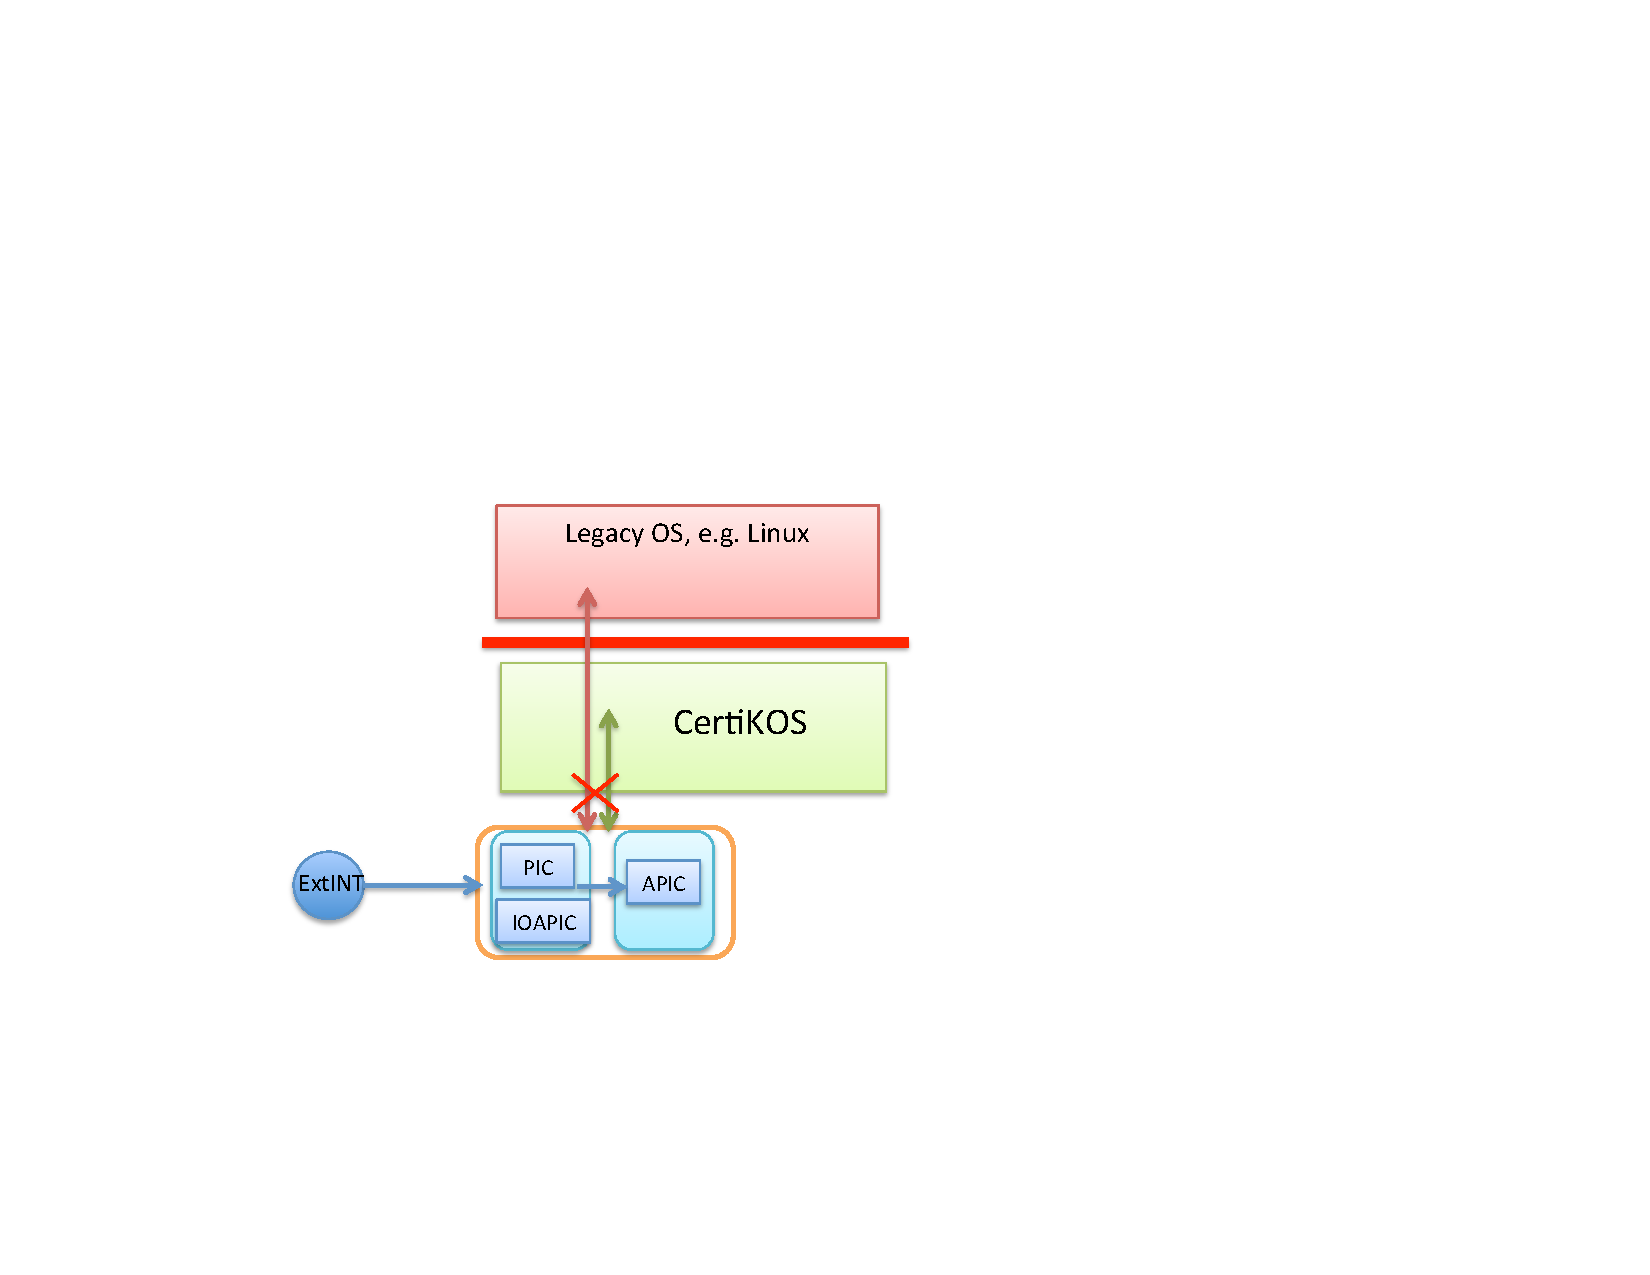
\includegraphics[width=0.5\textwidth]{conflict_pic}}
 \caption{Conflicts on Interrupt System } \label{fig:conflict}
\end{figure}


\subsubsection{Overview of Interrupt Virtualization in CertiKOS}

All these physical interrupt related chips are managed by CertiKOS, while a virtualized PIC is provided to the guest domain.     In current CertiKOS, it only supports PIC based interrupt in the guest domain.  As shown in Figure \ref{fig:vpic},  CertiKOS will get all interrupt signals, and it determines whether this interrupt should be handled by itself or guest.   The interrupt for the guest domain are supported by the VPIC.  VPIC simulates an i8259 chip for the guest domain and it records the VPIC setting for the guest domain.  
\begin{figure}[!ht]
 \centerline{
 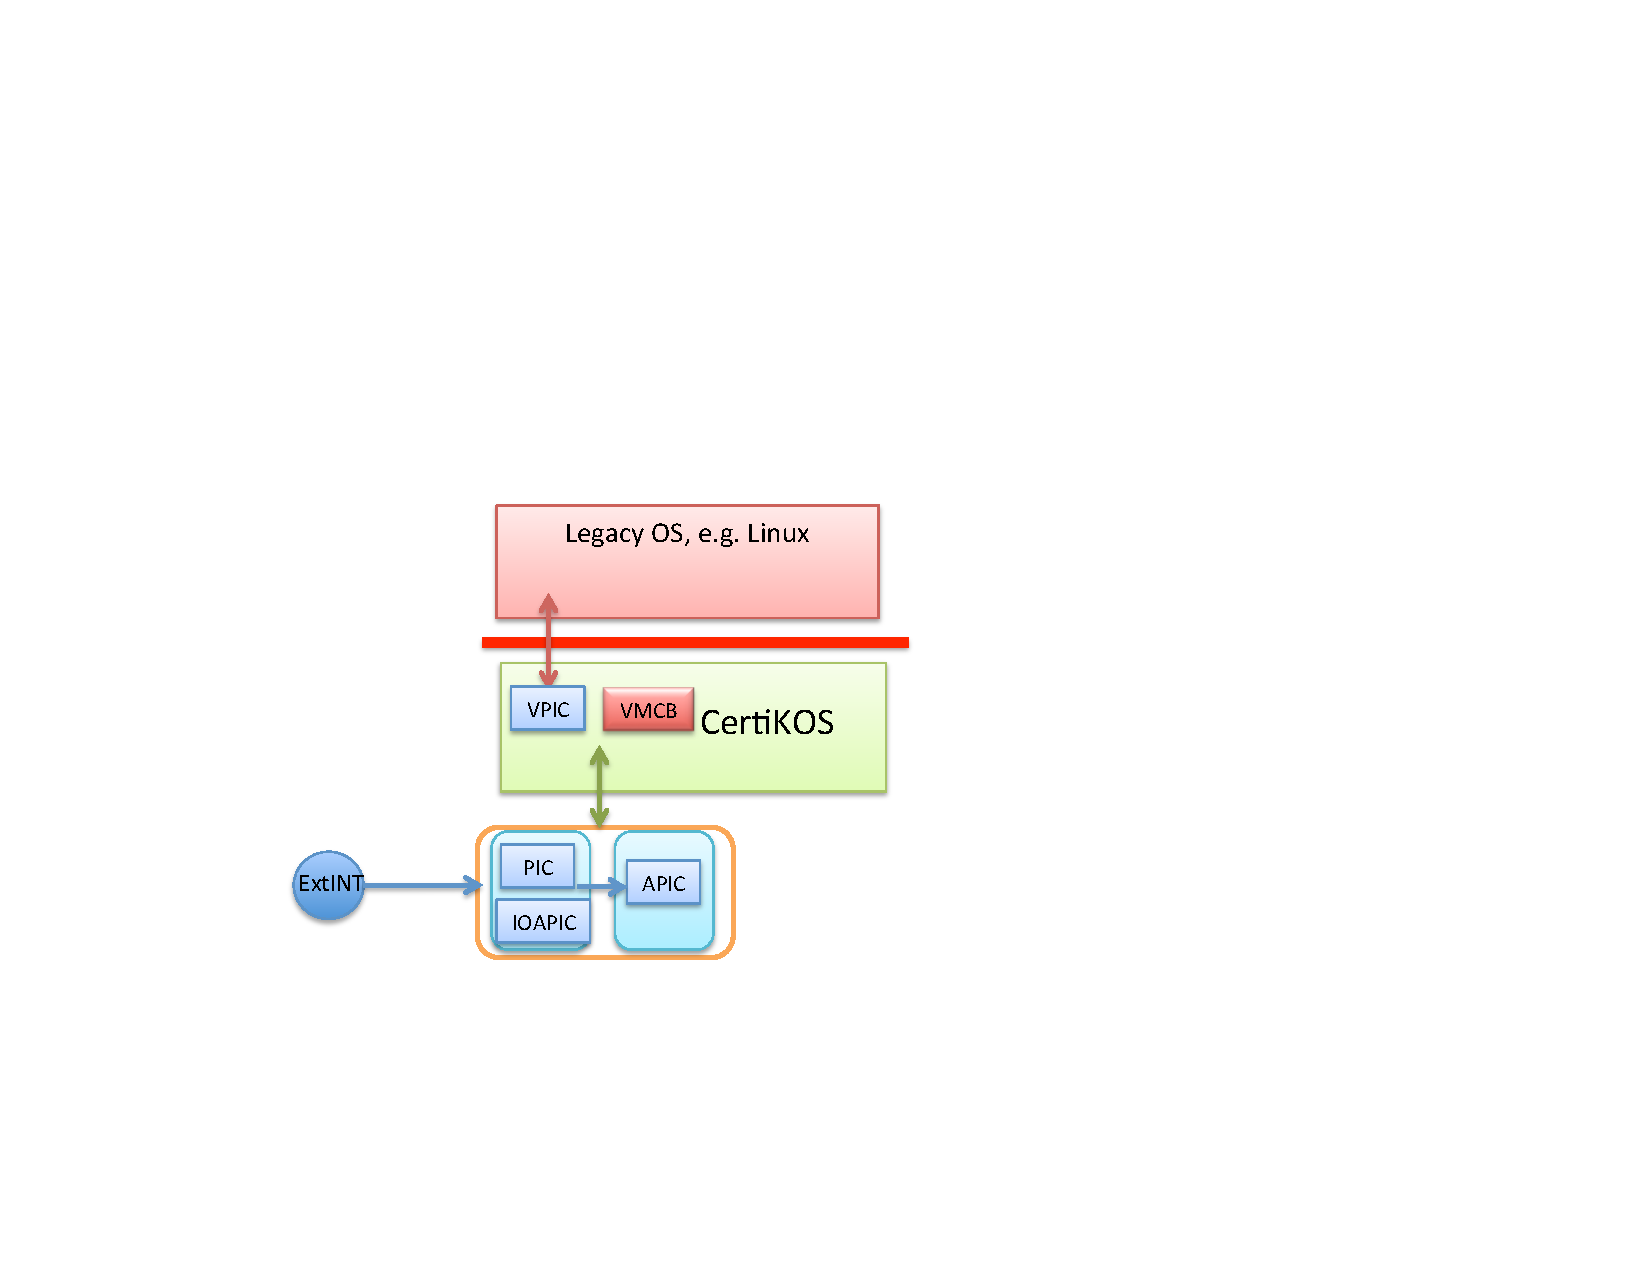
\includegraphics[width=0.5\textwidth]{vpic}}
 \caption{Interrupt Virtualization based on VPIC in CertiKOS} \label{fig:vpic}
\end{figure}

In CertiKOS, there are two situations for interrupt handling: (a)  CertiKOS runs on the physical core; (b) Guest OS runs on the physical core.   The interrupt handling for these two situations are corresponding to these two parts in Figure \ref{fig:vpic2}. When CertiKOS codes execute on the core, the interrupt will be directly handled by CertiKOS. When guest OS runs on the core, the CertiKOS intercepts the interrupt, and then this interrupt request will be identified by CertiKOS. After confirming that this interrupt is for the guest,  CertiKOS checks the status of guest OS and injects the interrupt into guest OS if guest OS is open for interrupt.  CertiKOS will also set the VPIC to record the interrupt request as being pending and the interrupt will be handled by the guest once it is interrupt enabled later.


\begin{figure}[!ht]
 \centerline{
 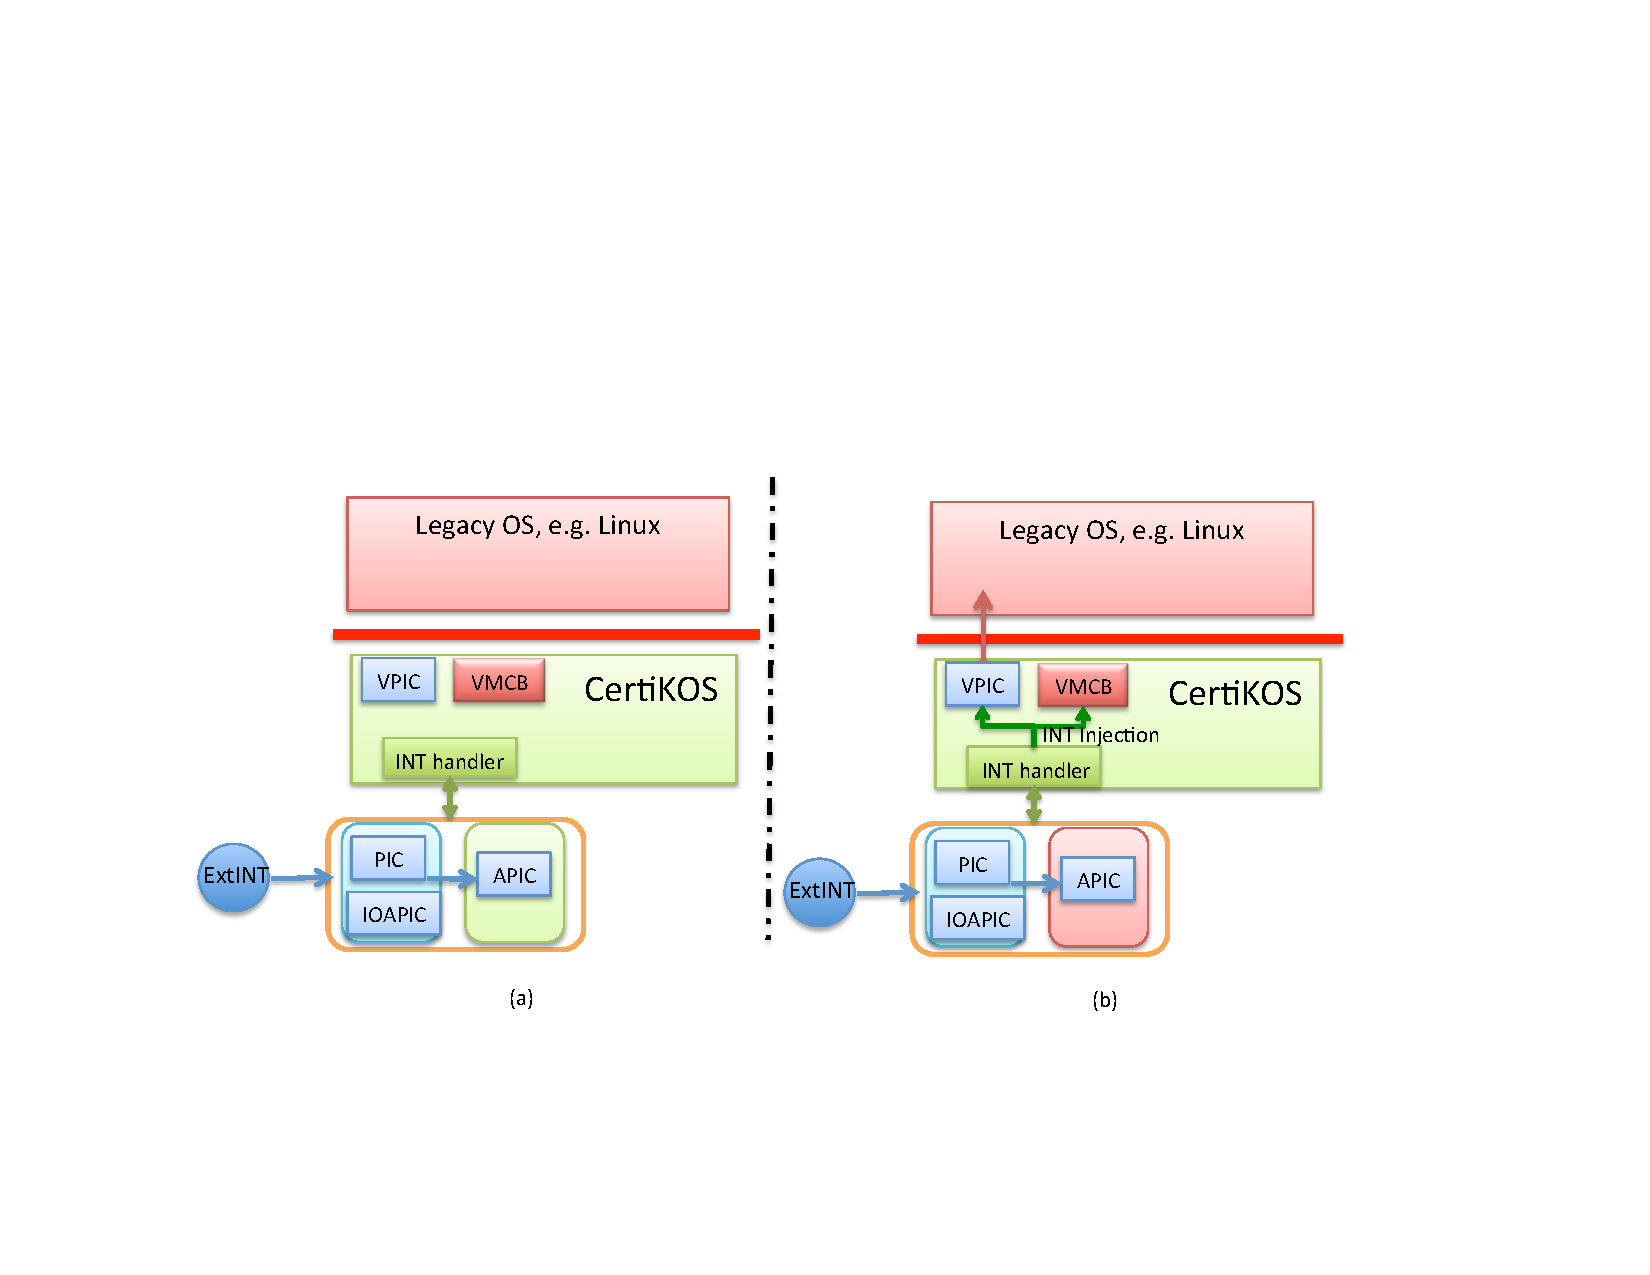
\includegraphics[width=0.8\textwidth]{interrupt_virtualization}}
 \caption{Interrupt handling in CertiKOS} \label{fig:vpic2}
\end{figure}






\subsubsection{Interrupt Chips}
\paragraph{PIC}
The 8259 Programmable Interrupt Controller (PIC) is one of the most important chips making up the x86 architecture.  The 8259 PIC controls the CPU's interrupt mechanism, by delivering  interrupt requests  to the processor in order.  PIC controls which interrupt request can be sent to the processor and how it is sent.  Each PIC chip has 8 inputs.  In modern IBM PC architecture, it usually provides two PIC chips in the master and slave mode.  So this kind of PIC chips can serve 15 interrupt sources. 



PIC chip can be accessed via two kinds of I/O port:  
\begin{itemize}
\item Command port: 0x20, 0xa0, 0x4d0
\item Data port: 0x21, 0xa1, 0x4d1
\end{itemize}

System first sends commands to the command port for selecting the operation for the following data object,  and then carries out the data operation via accessing the data port.   

There are two kinds of operations on PIC: Initialization command and  operation command. For the specification of these commands, please check the 8259 programmable interrupt controller specification \cite{PIC}. 

PIC has an interrupt mask register to control the enable/disable of interrupt delivery.  If PIC wants to not accept a specified interrupt source, it simply umask that bit  by setting it as 0. Otherwise, PIC can mask that bit by setting it as 1. 



\paragraph{}
To support interrupts in multi-processor interrupt management,  Local Advanced Programmable Interrupt Controller  (LAPIC)and I/O Advanced Programmable Interrupt Controller (IOAPIC) were introduced.


\paragraph{IOAPIC}
IOAPIC  consists of a set of interrupt input signals, a 24-entry by 64bit Interrupt Redirection Table, programmable registers, and a message unit for communication with APIC.I/O
devices inject interrupts into the system by asserting one of the interrupt lines to the IOAPIC. The IOAPIC
selects the corresponding entry in the Redirection Table and uses the information in that entry to format an
interrupt request message. Each entry in the Redirection Table can be individually programmed to indicate
edge/level sensitive interrupt signals, the interrupt vector and priority, the destination processor, and how the
processor is selected (statically or dynamically). The information in the table is used to transmit a message to
other APIC units (via the APIC bus).


Two of the registers: IOREGSEL-- I/O Register Select Register and IOWIN--I/O Window  Register, are located in the CPU's memory space and are used to indirectly access the other APIC registers as
described in Section 3.0 of IOAPIC specification \cite{IOAPIC}.  The read and write operations on other registers work based on these two registers.

I/O Redirection Table Registers record the delivery methods for each interrupt inputs.    The configuration of interrupt delivery mode include interrupt Vector, Delivery mode, Destination mode, Interrupt Mask, Trigger Mode, etc.  For more details, please check the specification of IOAPIC \cite{IOAPIC}. 

System can use more than one IOAPIC.

\paragraph{LAPIC}
Local APIC performs two primary functions for the processor: 
\begin{itemize}
\item It receives interrupts from the processor�s interrupt pins, from internal sources
and from an external I/O APIC (or other external interrupt controller). It sends
these to the processor core for handling.
\item In multiple processor (MP) systems, it sends and receives interprocessor
interrupt (IPI) messages to and from other logical processors on the system bus.
IPI messages can be used to distribute interrupts among the processors in the
system or to execute system wide functions (such as, booting up processors or
distributing work among a group of processors).
\end{itemize}

LAPIC also has a set of registers which are mapped to the physical memory address region: 0xFEE00000-0xFEE003F0. The configuration of these registers control the mode of interrupt message passing from APIC to processor. For the configuration details, check APIC specification in AMD and Intel specification \cite{AMD64, Intel64}. 


\subsubsection{Interrupt Modes}
Interrupt chips can work in different modes. Two modes are involved in CertiKOS: PIC mode for guest domain and APIC mode for CertiKOS. The purpose of interrupt virtualization is trying to provide PIC mode in Guest, while keeping APIC mode in CertiKOS.

\paragraph{PIC mode for Guest}
We first try to support guest domain with only PIC interrupt mode. The PIC interrupt mode is shown as in Figure \ref{fig:picmode}.   The doted line in the figure means the delivering path of interrupt signals. Only PIC is configured to serve as the interrupt controller, while other chips are not used. For more details, please check Section 3.6.2.1 in \cite{MP}.

\begin{figure}[!ht]
 \centerline{
 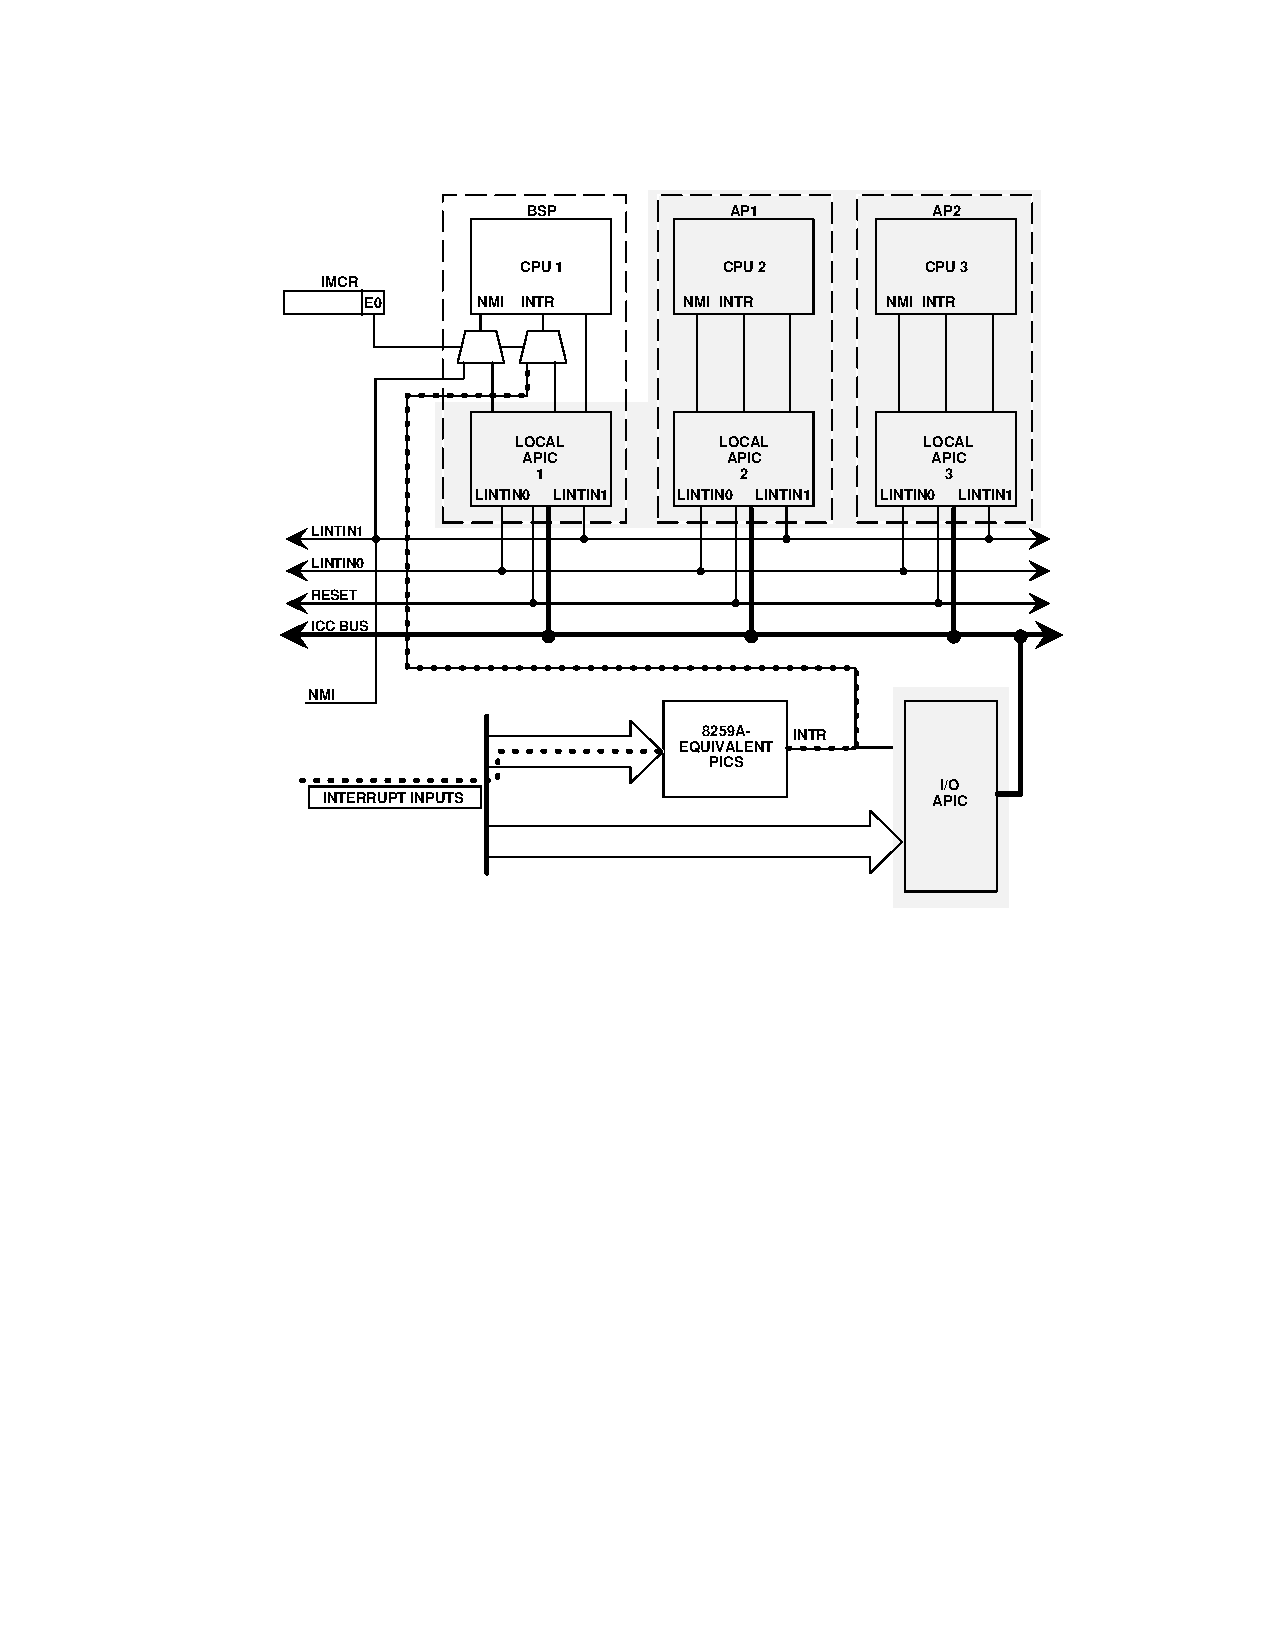
\includegraphics[width=0.9\textwidth]{pic_mode}}
 \caption{PIC interrupt mode} \label{fig:picmode}
\end{figure}

\paragraph{APIC mode}
In MP specification \cite{MP}, APIC mode is named as symmetric I/O mode (Section 3.6.2.3 in \cite{MP}). The configuration of interrupt chips in APIC mode is shown as Figure \ref{fig:mixedmode}.  In APIC mode, processors use LAPIC to get interrupt signals.  It is still possible to use PIC in APIC mode, which results a mixed mode. In mixed mode, both IOAPIC and PIC can serve as external interrupt controller.  In current implementation, PIC is simply masked to not accept all external interrupts and IOAPIC is used to handle external interrupt signals.


% In recent years, these latest hardware platforms have already employed the ACPI specification for providing MP configuration \cite{ACPI4}.
\begin{figure}[!ht]
 \centerline{
 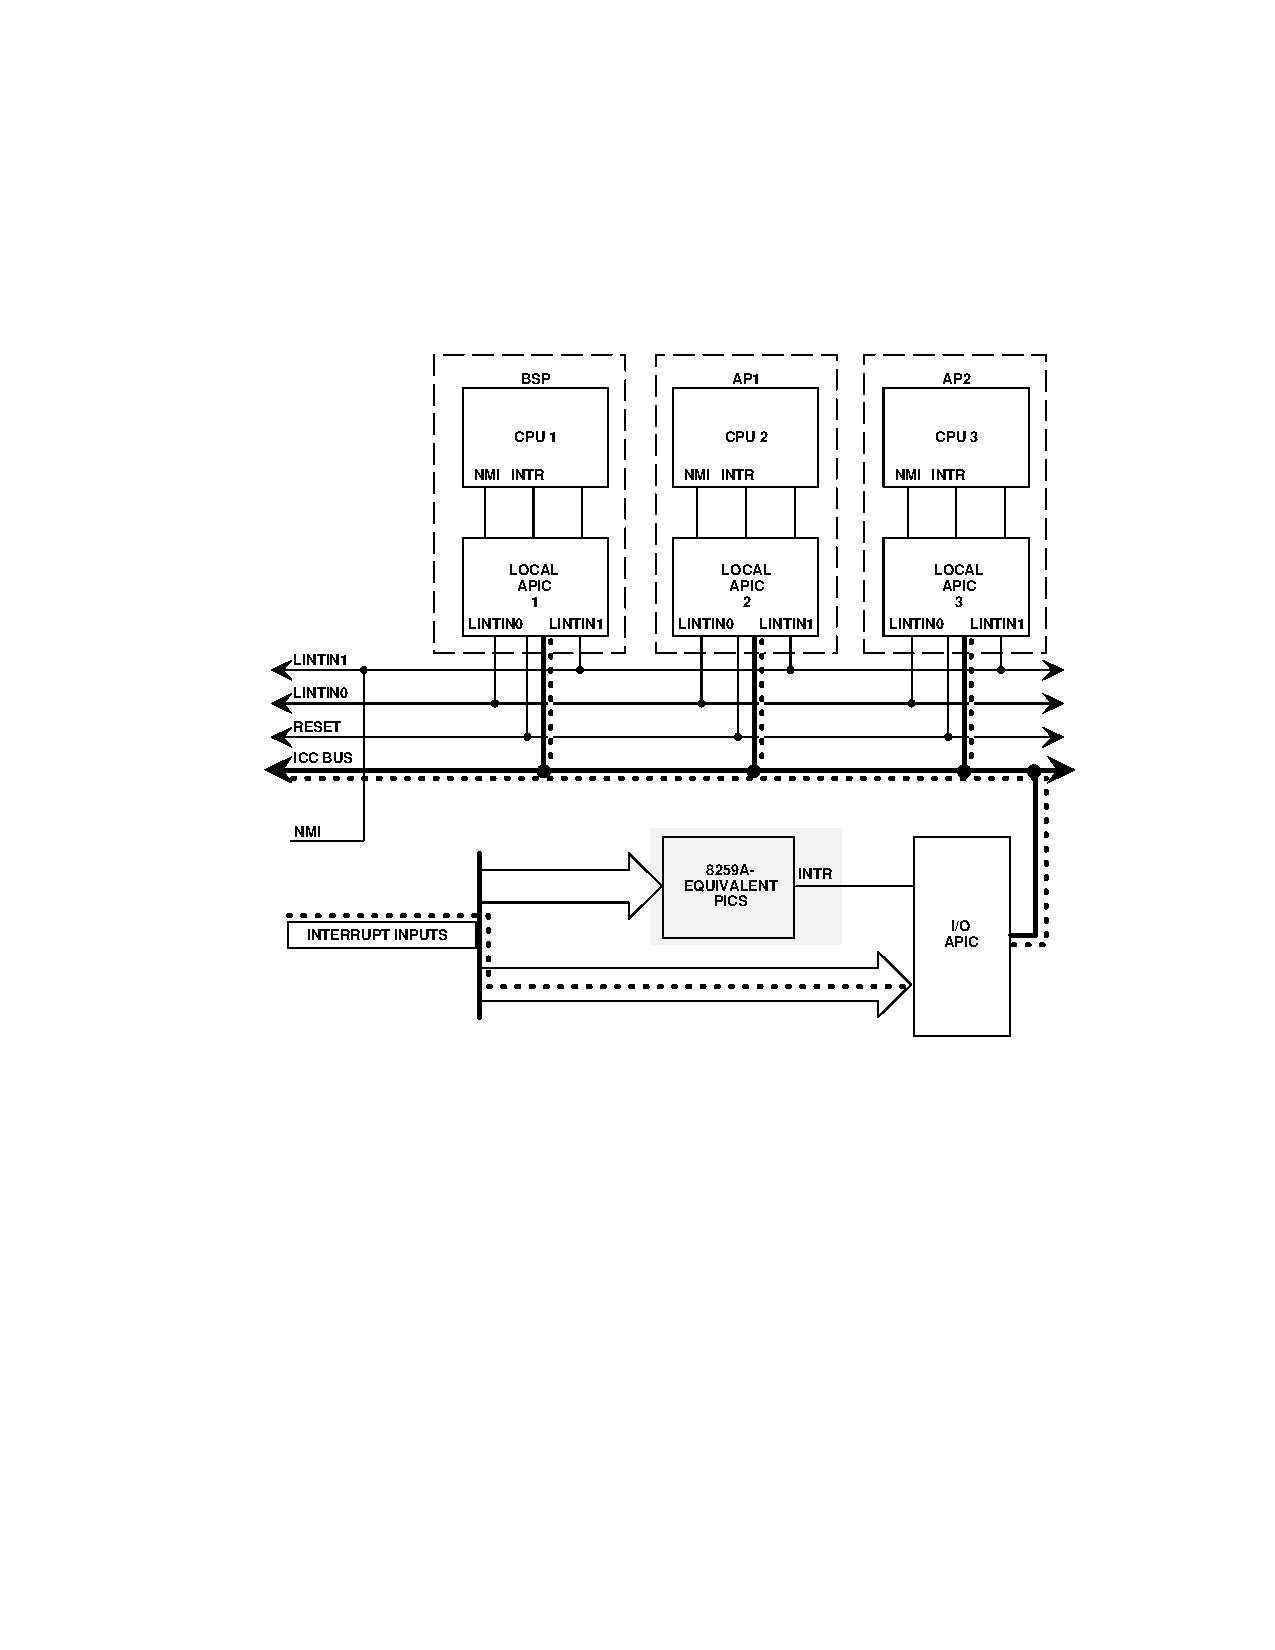
\includegraphics[width=0.9\textwidth]{mixed_mode}}
 \caption{APIC mode} \label{fig:mixedmode}
\end{figure}


\subsubsection{IO Port Interception for PIC Virtualization}
VPIC is implemented via intercepting IO operations in CertiKOS.   In PIC mode,  guest OS usually access PIC chip via following IO port: 0x20, 0x21,  0xa0, 0xa1,  0x4d1, 0x4d0.  All I/O operations on these ports are intercepted and redirected to VPIC. VPIC will handle these I/O operations the same as physical PIC. 



%\paragraph{List of critical devices}
%By enabling the interception of all IO accessing,  we noticed that following IO ports are accessed by the guest domain when it boots ttyLinux with Grub:
%\begin{itemize}
%\item PIC: 0xa0 0x20 0x21
%\item 0xed
%
%\item CGA: 0x3d4 0x3d5
%\item PCI:  0xcf8 0xcfc
%\item 0x1020
%%\end{itemize}
%
%By Intercepting IO operations on these ports, we can implement the simulation of these devices while handling vm exit events.

 We currently introduce IO handling in the CertiKOS kernel, as  in Figure \ref{fig:iohandling}.  When the guest OS is going to access the PIC, CertiKOS intercepts the operation. It either sets the simulated data structure with these setting from guest OS, or returns the configuration from these simulated data structure to the guest OS.

\begin{figure}[!ht]
 \centerline{
 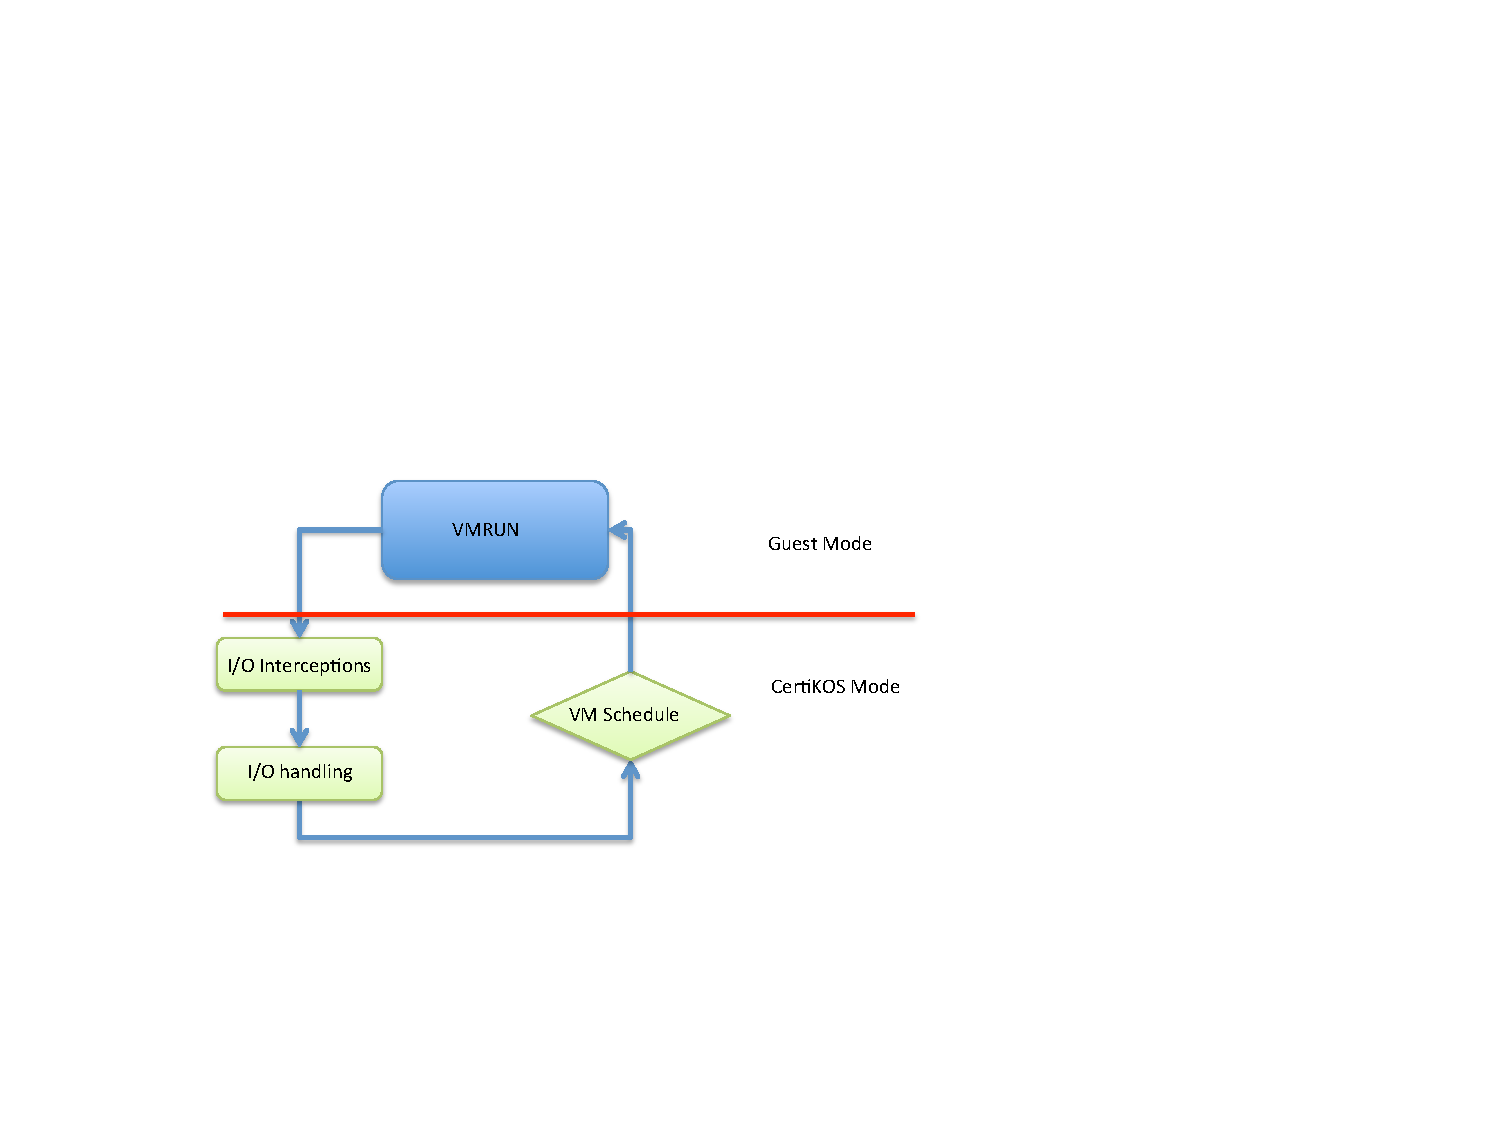
\includegraphics[width=0.7\textwidth]{IO_handling}}
 \caption{IO handling for VM at kernel mode} \label{fig:iohandling}
\end{figure}

For the long term, we will move IO handling up to application layer,  as in Figure \ref{fig:iohandling2}.
\begin{figure}
 \centerline{
 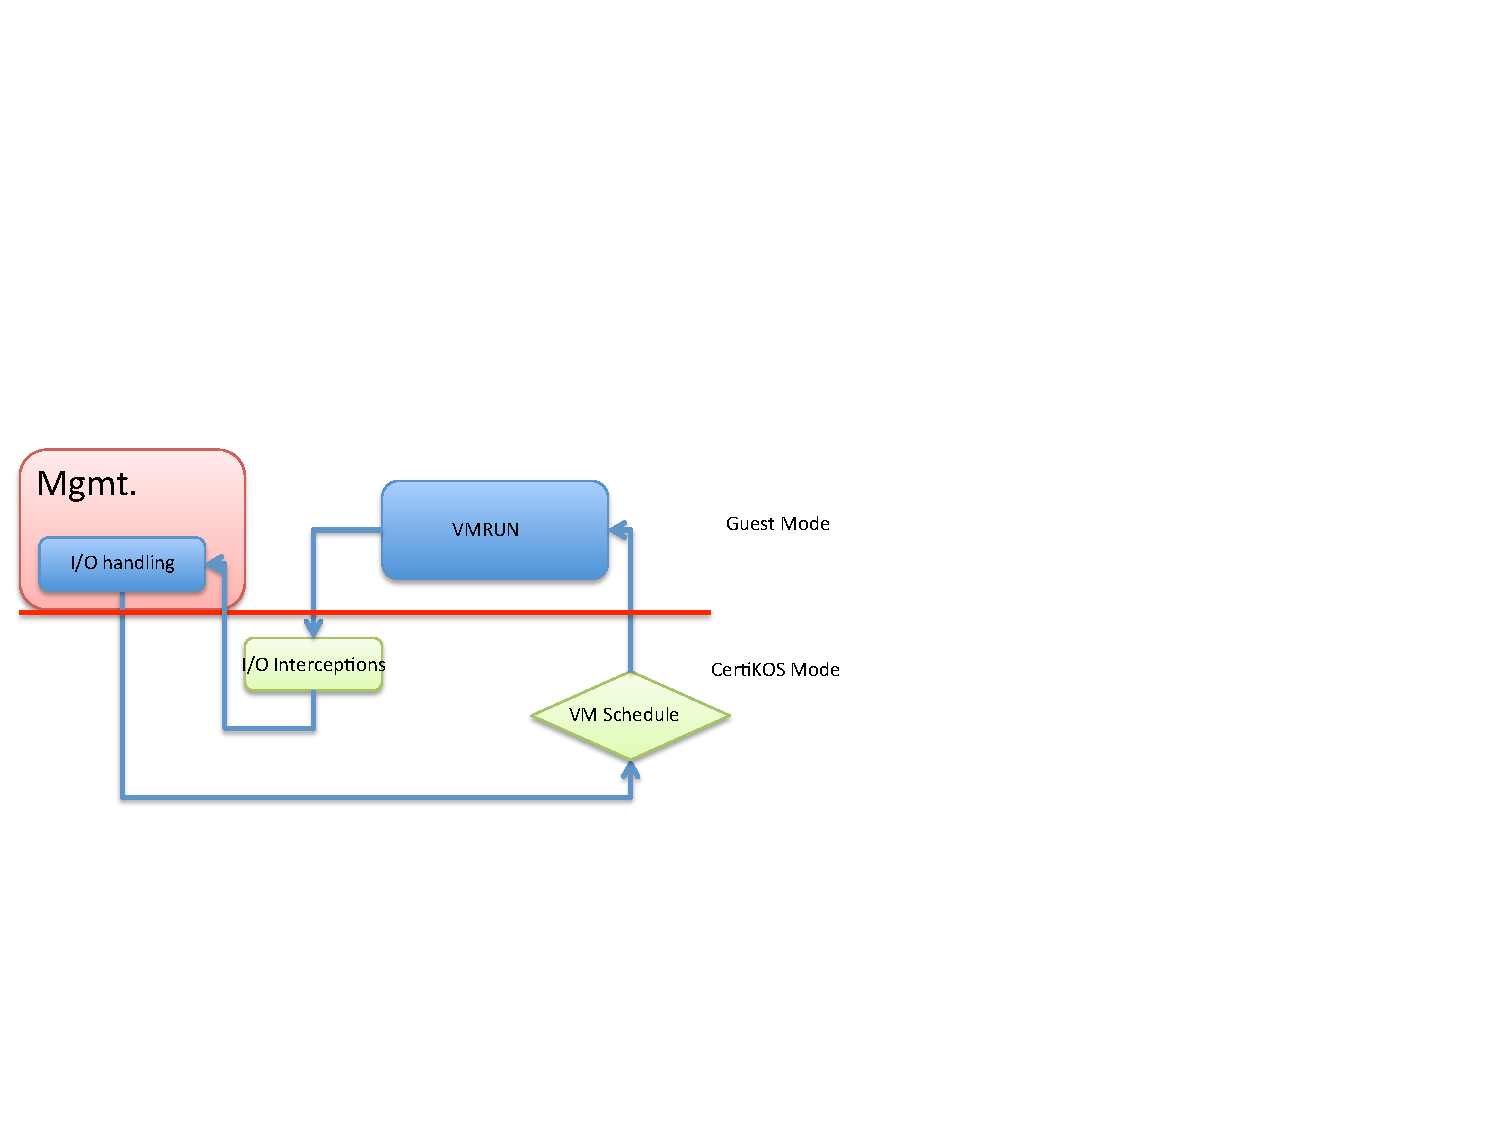
\includegraphics[width=0.7\textwidth]{IO_handling2}}
 \caption{IO handling for VM at guest mode} \label{fig:iohandling2}
\end{figure}


\subsubsection{Interrupt Injection}
As shown in Figure \ref{fig:vpic2}, when guest OS runs on the physical processor core,  external interrupts will be intercepted by CertiKOS.   CertiKOS will get the IRQ number in the trap routine.  Then CertiKOS queries the VPIC to get the corresponding VIRQ in the guest domain and injects the interrupt with this VIRQ.  For an interrupt injection, CertiKOS  fills the EVENTINJ field of VMCB and raises an  interrupt request in the VPIC.   If the guest is able to handle the interrupt, it will immediately handle this injected interrupt.  If not, the interrupt in the VPIC will be kept as being pending until guest handles it.

%\subsubsection{Interrupt Handling}
%\label{subsec:interrupthandling}
%As CertiKOS and Guest OS share some of these physical devices, like keyboard, it requires the CertiKOS to handle some external interrupts for the Guest OS to correctly handle interruption events.
%
%  \begin{figure}[!ht]
% \centerline{
% \includegraphics[width=0.6\textwidth]{interrupt_handle}}
% \caption{Interrupt handling for guest OS} \label{fig:interrupthandle}
%\end{figure}
%As in Figure \ref{fig:interrupthandle}, CertiKOS intercepts the interrupt events for handling these external interrupts for guest OS.   First, CertiKOS will set the interception setting of the guest domain (Step 1 in Figure \ref{fig:interrupthandle}).  Once the guest has these specified interrupts, the CertiKOS will intercept the event and return the correct IRQ handler for the guest OS (Step 2 in Figure \ref{fig:interrupthandle}). Then the guest can continue its execution for handling the interrupt.
%
%Now we are implementing and testing  the code of interrupt handling for guest OS.



\subsection{Enable CertiKOS on Physical Platform}
The previous versions of CertiKOS are mostly running on SimNow. We leverage the debugging function of SimNow to  search and fix the errors and bugs in CertiKOS. However, the real physical platforms may have some subtle differences from SimNow, which cause CertiKOS cannot function properly in the real world. Thus, an indispensable part of our work is to port and test CertiKOS on the physical platform. The first two phases is to boot CertiKOS on the physical platform, and boot a guest OS on CertiKOS. In the future, we need to do more test and fixes to let the CertiKOS and the guest OS work properly other than just bootstrap. 

\paragraph{Boot CertiKOS}
Current version CertiKOS must work on a SMP platform, because it requires the management OS and client applications run on different processor cores. Thus, CertiKOS checks whether it is running on a SMP platform when booting. If not, CertiKOS will not work properly, {\it e.g.} panic on UP platform. Previous versions of CertiKOS follow Intel Multiprocessor Specification\cite{MP} to detect and mange multiprocessors, {\it i.e} through {\it MPT}({\it MultiProcessor Table}). However, \cite{MP} is actually deprecated and lots of recent machines do not provide MPT any more. CertiKOS can not boot on these machines consequently. The resolution is turning to {\it ACPI}({\it Advanced Configuration and Power Interface}), which is the new standard. The legacy MPT code now works as a fallback method for the old platforms follow Intel Multiprocessor Specification other than ACPI. After fixing this error, CertiKOS can now boot on our physical machine. Still we need to test on more physical platforms.

\paragraph{Boot Guest OS (TTY Linux)}
The subtle differences between SimNow and the physical platform also cause the failure of booting TTY Linux as the guest OS in the real world. After bootloader loads the linux kernel, the kernel will first detect the hardware, set up the memory layout for the physical memory, and then create the data structures for paging, etc. Then is the non-architecture specific booting procedure, {\it i.e.} setting up interrupts, perform memory configuration and load the initial RAM disk. In the end of this procedure, the kernel will start an idle task (a user thread).

Currently TTY Linux can pass all architecture specific booting procedure, but it maybe stuck at some places in the non-architecture specific booting procedure, such as the point starting the idle task. Though the later procedure is named as {\it non-architecture specific}, some functions invoked in this procedure still depend on the hardware. Take the starting idle task as an example. The primary function of idle task is ``idle''. However, the implementation of ``idle'' depends on the features of the processors. In this case, the feature is called {\it C1E}. The hardware configuration we use in SimNow does not support C1E. While the real processors have this feature, so CertiKOS is stuck in the real world, though it works properly in the simulator.

We follow such steps to resolve these problems:
\begin{enumerate}
\item Disable the feature caused the problem. If it works, then go to the next problem; otherwise, take the second step.
\item Simulate the feature in SimNow, {\it i.e.} either implementing the feature in SimNow, or allowing the guest OS to access the feature of the hardware.
\end{enumerate}




%\subsubsection{PCI}
%For simplicity, we are now modifying the MP configuration for the guest OS and make guest think that there is no PCI devices.
%However, in future, if CertiKOS needs to share PCI devices between the host and guest, we have to implement the simulation of PCI bus and schedule the device accessing.
%
%We are now testing the codes and setting for PCI simulation for the Guest.

\subsection{Working problem}

To support legacy guest as guest applications, we are working on interrupt virtualization in CertiKOS.  We introduce virtualized PIC (Programmable interrupt Controller)  to support guest domain, while keeping the physical PIC and APIC available for the host (CertiKOS).  We are countering two problems for debugging the interrupt virtualization.  

\subsubsection{Read Error of GRUB in Guest Domain}
As shown in Figure \ref{fig:readerror},  with VPIC, the Guest domain has a Read Error at the GRUB stage.    By following the execution GRUB and BIOS,  GRUB hangs there for the response of disk read.  This is the same situation for booting guest domain without VPIC, if CertiKOS does not reset the physical chip before booting into the guest domain.   
\begin{figure}
 \centerline{
 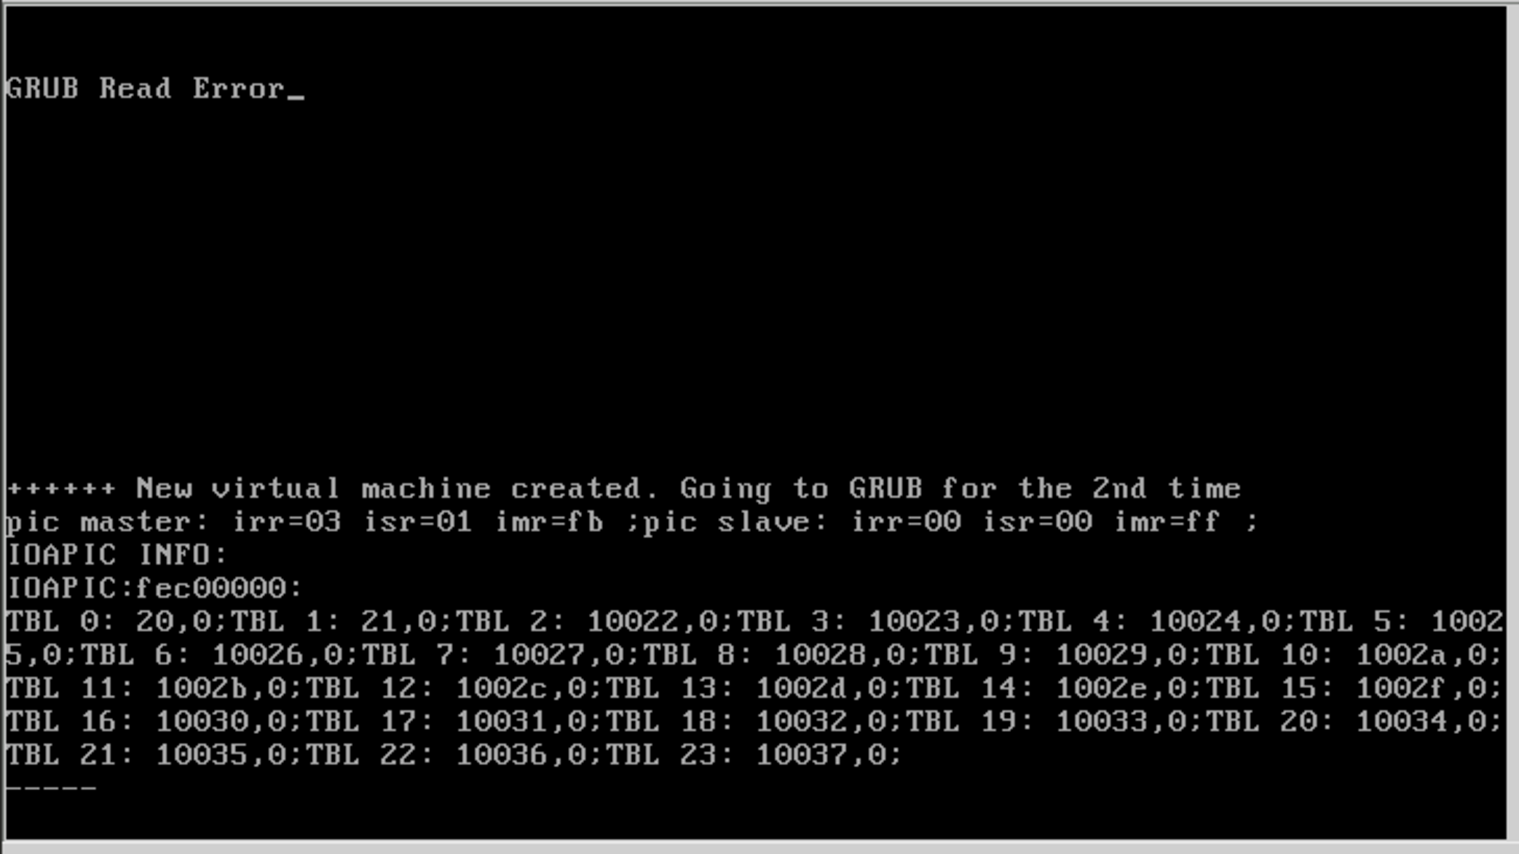
\includegraphics[width=0.7\textwidth]{read_error_screen}}
 \caption{Read Error while  booting guest  domain with VPIC } \label{fig:readerror}
\end{figure}

As we discussed in the meeting, this  is probably caused by the setting of BIOS.  We are now replacing the Host BIOS with seaBIOS to control the whole software stack in Guest domain. 
%How to virtualize the interrupts based on VPIC  for the guest OS? we are trying to confirm and  check our understanding by  examining the QEMU-KVM and test cases on CertiKOS.  Some of these points that need be further confirmed are presented in following paragraphs.
%  \begin{figure}[!ht]
% \centerline{
% 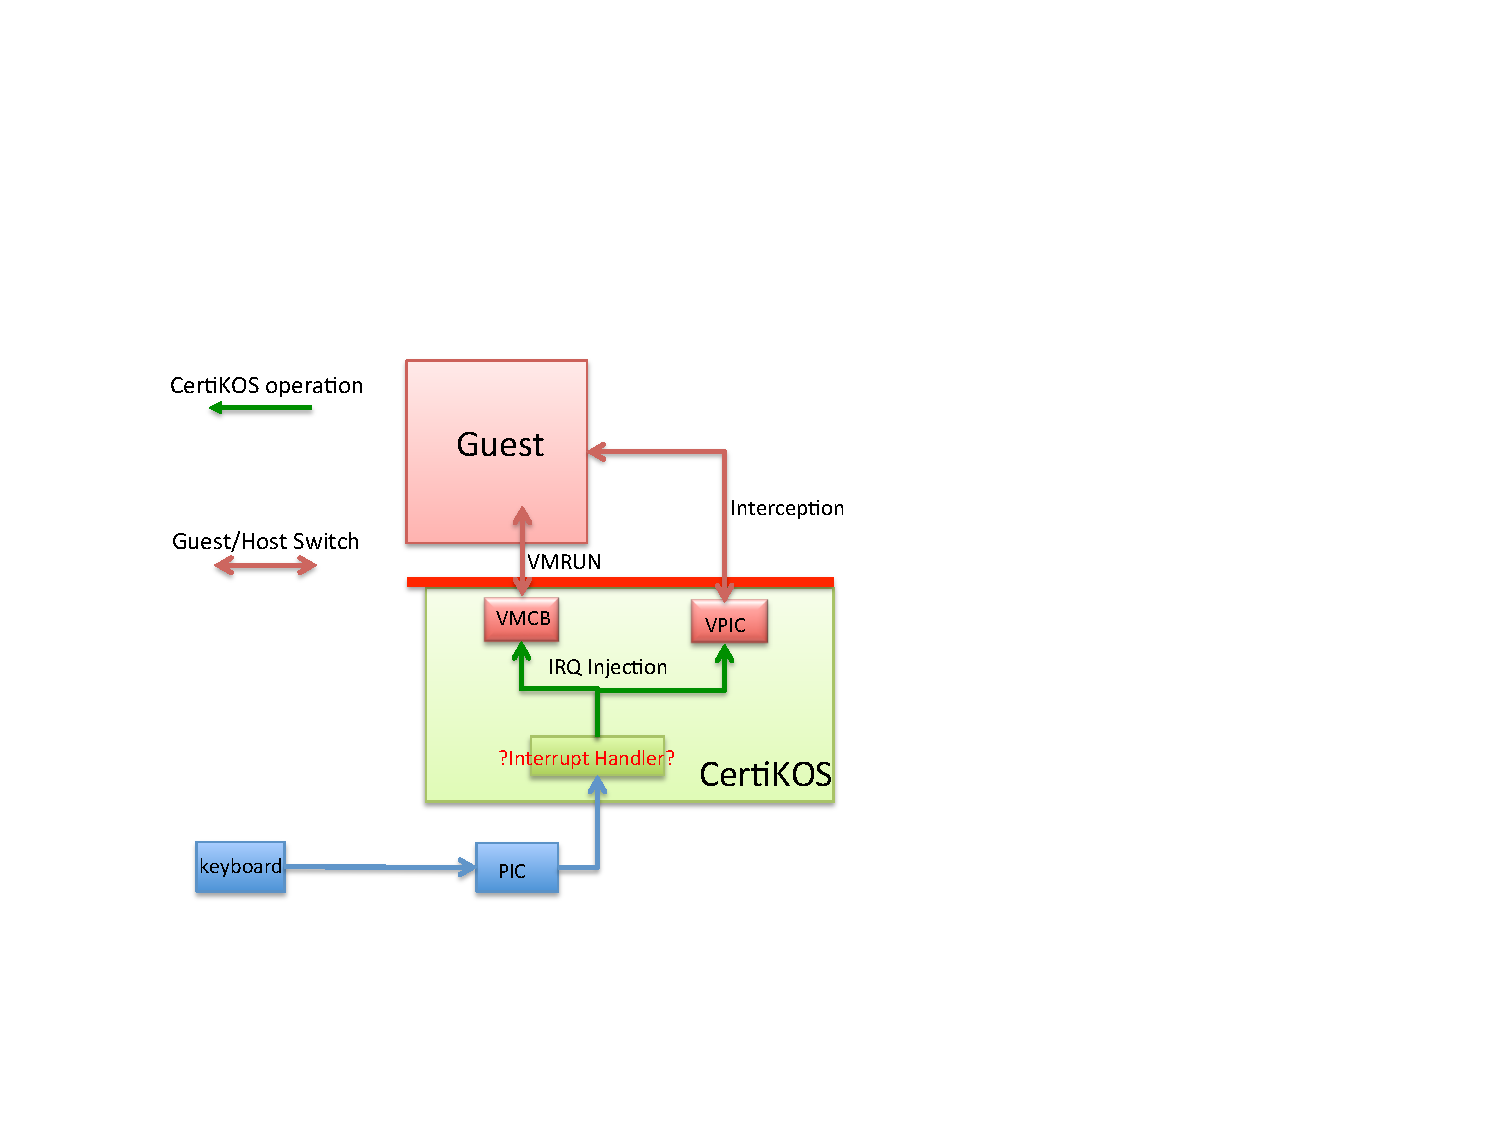
\includegraphics[width=0.6\textwidth]{interrupt_injection}}
% \caption{PIC Interrupt virtualizing for guest OS} \label{fig:interruptinjection}
%\end{figure}
%
%When a physical device interrupt happens, like keyboard,  CertiKOS checks whether this is for the guest (By checking the interrupt pending status of the guest). If it is, then CertiKOS will inject Interrupt into guest by setting VMCB of the guest os.   Whether our understanding about virtualizing interrupts correct? 
%
%Where is the right place for the IRQ injection in CertiKOS? The CertiKOS interrupt handler?  In another word, How can CertiKOS separate  external interrupt events for its own and guest OS? 
%
%In AMD SVM specification, it introduces a kind of interception for Virtual Interrupts in Guest OS.   I am still not sure whether this type of virtual interrupt is what we want to implement (interrupt virtualization),  or  it refers to the guest OS  interrupts of protected mode virtual interrupt. If it is for interrupt virtualization, how can we leverage it to help the PIC related interrupt simulation?  We are still checking the implementation of KVM to study its usage. 

\subsubsection{ Delivering external interrupt to guest domain on physical platform}



On the physical platform,  the guest domain is able to boot into GRUB menu and some further into the ttyLinux initialization stage.  However, the guest domain can not get external interrupts, like keyboard.  We think that this problem is probably also caused by the BIOS configuration. 






\subsection{Plan for Next Stage}
We are now mostly working on finish following tasks : 
\begin{itemize}
\item boot ttyLinux as guest OS with CertiKOS on Physical Platform
\item boot ttyLinux with simulated PIC interrupt mode  in CertiKOS
\item intercept  critical operation in ttyLinux
\end{itemize}


%\section{Related Work}
%
%\subsection{Interrupt simulation in QEMU and KVM}
%$kvm\_arch\_pre\_run$



\bibliographystyle{plain}
\bibliography{certikos}


\end{document}
